% !TeX program = lualatex
% !TeX encoding = utf8
% !BIB program = biber
% !TeX spellcheck = uk_UA

\documentclass[print]{MastersDiploma}
\usepackage{caption}
%\usepackage{adjustbox}

%================================================ ФАЙЛИ ЛІТЕРАТУРИ ======================================
%
\addbibresource{Bibliography/bibliography.bib}
%
%=======================4=================================================================================


%=========================================== ІНФОРМАЦІЯ ПРО ДИСЕРТАЦІЮ ==================================
%
\author{Макарчук Богдан Олексійович}
\authorinitials{Б.~О.~Макарчук}
\kurs{6}
\grupa{ФФ-11мн}
\title{Оцінка параметрів концепту гібридної електрохімічної силової установки літального апарата}
\kerivnyk{доцент, к.ф.-м.н. Пономаренко С.~М.}
\konsultant{}
\retsenzent{с.н.с., к.т.н. Доник Т.~В.}
\udc{536.8}
%--------------------------------------------------------------------------------------------------------
\univapproved{07}{червня}{\the\year~р}{1459-с} % затверджені наказом по університету
\submission{10}{червня}{\the\year~р.} % термін подання студентом роботи
\issuing{10}{вересня}{2020~р.}% дата видачі завдання
%--------------------------------------------------------------------------------------------------------
\searchobject{Термогазодинамічні процеси та кінетика горіння паливної суміші в камері РРД за присутності присадки калію.} % Об'єкт дослідження
\predmet{Баланс параметрів паливної суміші та іонізуючої присадки для збільшення питомого імпульсу досліджуваного двигуна.}% Предмет дослідження
\tasks{Змоделювати процес горіння палива у камері згоряння РРД за заданих геометричних параметрів, витрати пального та окиснювача та параметрів системи охолодження камери; Провести моделювання за допомогою програмного комплексу ANSYS; Провести моделювання вищеозначеного процесу за присутності заданої концентрації частинок калію; порівняти параметри потоку без присадки та за її присутності; отримати вихідні параметри тяги та питомого імпульсу досліджуваного двигуна, спираючись на параметри конкретного РРД та відповідної йому за геометричними та масовими параметрами МПД-установки; порівняти їх із показниками вихідного РРД.}%Перелік завдань
\illustrations{презентація --- 16 аркушів А4}
\publications{Оцінка параметрів концепту гібридної електрохімічної рушійної установки літального апарата} % Публікації


\specialnist{105  <<Прикладна фізика та наноматеріали>>}
%
%========================================================================================================


\begin{document}

%========================================================================================================
%
%									      Вставка титулки та інших супровідних документів
%
%========================================================================================================

\pagestyle{empty}
\titlepage
%========================================================================================================
%
%										            Taskpage
%
%========================================================================================================


\newgeometry{
	showframe,
	footskip=0cm,%
	headsep=0cm,%
	top=1cm, %поле сверху
	bottom=1cm, %поле снизу
	left=2cm, %поле ліворуч
	right=1cm, %поле праворуч
}

\begin{spacing}{1.1}

\begin{center}{%
	\bfseries
	{Національний технічний університет України}\\
	{<<Київський політехнічний інститут імені Ігоря Сікорського>>}%
    }\\

	Навчально-науковий Фізико-технічний інститут\\
	Кафедра фізики енергетичних систем\\
\end{center}

\noindent Рівень вищої освіти --- другий (магістерський)\\
\makeatletter
\noindent Спеціальність  \@specialnist
\makeatother

\vspace*{1.5em}%
\noindent%
\hfill\begin{minipage}[t]{0.5\linewidth}
	<<ЗАТВЕРДЖЕНО>>\\
	Завідувач кафедри\\
	\mfield{0.2\linewidth}{}{}{}{(підпис)} \mfield{0.75\linewidth}{}{}{Монастирський~Г.~Є.}{(ініціали, прізвище)}\\
	\mfield{0.15\linewidth}{<<}{>>}{}{} \mfield{0.5\linewidth}{}{}{}{}~2023~р.\\
\end{minipage}

\begin{center}
	{\Large\bfseries ЗАВДАННЯ}\\
	{\bfseries на магістерську дисертацію студенту}\\
\end{center}
\makeatletter%
\noindent\mfield{0.8\textwidth}{}{}{Макарчуку Богдану Олексійовичу}{(прізвище, ім’я, по батькові)} \mfield{0.2\textwidth}{}{}{}{(підпис)}
\makeatother%

\begin{enumerate}[label*=\arabic*., labelindent=0pt, itemindent=0cm]
	\makeatletter%
	\item Тема роботи: \@title,

	\noindent\mfield{1\linewidth}{науковий керівник роботи}{}{\@kerivnyk}{(прізвище, ім’я, по батькові, науковий ступінь, вчене звання)},\vspace{-3mm}\\

	\noindent затверджені наказом по університету від \@univapproved
	\item Термін подання студентом роботи \@submission
	\item Об’єкт дослідження: \@searchobject
	\item Предмет дослідження: \@predmet
	\item Перелік завдань, які потрібно розробити: \@tasks
	\item Орієнтовний перелік ілюстративного матеріалу: \@illustrations

\end{enumerate}



\restoregeometry


\end{spacing}
%\afterpage{%
%	\newgeometry{<options>}
%	% material for this page
%	\clearpage
%	\restoregeometry
%}

%========================================================================================================
%
%										            Taskpage
%
%========================================================================================================


\newgeometry{
	showframe,
	footskip=0cm,%
	headsep=0cm,% 
	top=1cm, %поле зверху
	bottom=1cm, %поле знизу
	left=1cm, %поле ліворуч
	right=2cm, %поле праворуч    
}

\begin{spacing}{1.1}
		
\begin{enumerate}[label*=\arabic*., labelindent=0pt, itemindent=0cm]
	\makeatletter%


%\clearpage
%
%\newgeometry{
%	a4paper,%
%	footskip=0cm,%
%	headsep=0.5cm,% 
%	top=2cm, %поле зверху
%	bottom=2cm, %поле знизу
%	left=1cm, %поле ліворуч
%	right=2cm, %поле праворуч
%}

\item[7]  Орієнтовний перелік публікацій: \@publications
\item[8] Консультанти розділів дисертації
	\noindent%
\begin{center}
		\small
\resizebox{\textwidth}{!}{%
\begin{tabular}{|c|c|r|r|}
	\hline
	\multirow{2}[4]{*}{Розділ} & \multirow{2}[4]{*}{\thead{Прізвище, ініціали та посада \\ консультанта}} &                     \multicolumn{2}{c|}{Підпис, дата}                     \\ \cline{3-4}
	                           &                                                               & \multicolumn{1}{c|}{завдання видав} & \multicolumn{1}{c|}{завдання прийняв} \\ \hline
	            %1              &                         \@konsultant                          &                                     %&                                     \\ \hline
	            2              &                         \@konsultant                          &                                     &                                     \\ \hline
	            3              &                         \@konsultant                          &                                     &                                     \\ \hline
\end{tabular}%
}
\end{center}
	
	\item[9] Дата видачі завдання \@issuing
	\begin{center}
		Календарний план
	\end{center}
\begin{center}
	\small%
\resizebox{\textwidth}{!}{%
\begin{tabular}{|c|l|c|r|}
	\hline
	\thead{№ \\ з/п} & \thead{Назва етапів виконання \\ магістерської дисертації} & \thead{ Термін виконання \\етапів проекту} & Примітка \\ \hline
	   1. & Опрацювання літератури за темою                 &            10.09.2020 - 31.10.2020               &          \\ \hline
	   2. & Написання літературного огляду                  &            01.11.2020 - 28.12.2020               &          \\ \hline
	   3. & Моделювання роботи РРД з присадкою калію           &            05.01.2021 - 18.03.2021               &          \\ \hline
%	   4. & Знаходження геометрично вигідного положення     &                                                  &          \\ \hline
	   4. & Написання другої частини дипломної роботи       &            19.03.2021 - 11.05.2021               &          \\ \hline
%	   6. & Варіювання подачі вторинного повітря            &                                                  &          \\ \hline
	   5. & Підготовка тез			                        &            11.05.2021 - 13.05.2021               &          \\ \hline
	   5. & Виступ на конференції                           &            14.05.2021                            &          \\ \hline
	   6. & Написання третьої частини дипломної роботи      &            15.05.2021 - 29.05.2021               &          \\ \hline
	   7. & Написання висновків                             &            30.05.2021 - 31.05.2021               &          \\ \hline
	   8. & Подання роботи на рецензування                  &            01.06.2021                            &          \\ \hline
	   9. & Підготовка доповіді та презентації              &            19.05.2023 - 22.05.2023               &          \\ \hline
	  10. & Подання роботи до захисту                       &            23.05.2023                            &          \\ \hline
\end{tabular}%
}
\end{center}
	
	\makeatother%
\end{enumerate}	

%\clearpage
%\newgeometry{
%	a4paper,%
%	footskip=0cm,%
%	headsep=0.5cm,% 
%	top=2cm, %поле сверху
%	bottom=2cm, %поле снизу
%	left=1cm, %поле ліворуч
%	right=2cm, %поле праворуч
%}
%\vfill
\vspace*{63mm}%
\noindent%
\makeatletter
\hfill\begin{minipage}[t]{\linewidth}
Студент\hfill\mfield{0.2\linewidth}{}{}{}{(підпис)} \mfield{0.4\linewidth}{}{}{\@authorinitials}{(Б.~О.~Макарчук)}\\	
Науковий керівник роботи\hfill\mfield{0.2\linewidth}{}{}{}{(підпис)} \mfield{0.4\linewidth}{}{}{С.~М.~Пономаренко}{(ініціали, прізвище)}
\end{minipage}
\makeatother
\restoregeometry

\end{spacing}


%\afterpage{%
%	\newgeometry{<options>}
%	% material for this page
%	\clearpage
%	\restoregeometry
%}

%========================================================================================================
%
%									      Вставка реферату
%
%========================================================================================================
% !TeX program = pdflatex
% !TeX encoding = utf8
% !TeX spellcheck = uk_UA
\restoregeometry
\begin{center}
	{РЕФЕРАТ}
\end{center}
%\totaltables~таблиць та

Пояснювальна записка дипломної роботи за обсягом становить   \pageref*{LastPage}~сторінки, містить \totaltables~таблиці та  \totalfigures~рисунків. Для дослідження було використано  \total{citenum}~бібліографічних найменувань.

%Робота присвячена питанню ефективного спалювання пилоподібного вугільного палива різного діаметру у суміші з газами, яка
%подається у проточний реактор. 

Метою роботи є доведення можливості поєднання РРД і МПД-прискорювача у межах однієї силової установки КА з точки зору процесів термо-, газодинаміки і фізики горіння шляхом умовного з'єднання камери згоряння РРД і МПД-канала і моделювання стабільної роботи двигуна у такій конфігурації. Предметом дослідження є аспекти роботи такої моделі, що визначають приріст питомого імпульсу двигуна, а саме вплив компоненти робочого тіла МПД-прискорювача на процеси, протікаючі у камері згоряння РРД.

Виконане числове моделювання потокiв робочого тiла рiдинного ракетного двигуна (РРД) заданих параметрiв (горюча сумiш газiв пiд високим тиском) i магнiтоплазмодинамiчного (МПД) прискорювача (iонiзуюча присадка металiчного дрiбнодисперсного калiю) та їх взаємодiї у межах одного робочого перерiзу. У ході аналізу результатів було з’ясовано, що профiлi температур i швидкостей дискретної фази (присадки) мають розподiл значень, близький до розподiлу параметрiв потоку РРД; досягається певна рiвновага мiж частинками й потоком, що впливає на результуючi робочi характеристики дослiджуваної схеми рушiйної установки.

Аналіз результатів проведеного моделювання показав, що МПД-компонент плазморідинного двигуна для компенсації малої витрати присадки за габаритів, не перевищуючих довжину камери досліджуваного РРД і маючи котушки технологічно досяжних параметрів має прискорювати потік струмами порядку 1...10 кА, що потребує підведення потужності порядку 2...20 МВт.

%\textbf{Мета.} Дослідити вплив розміру вугільних частинок на процес їх горіння у суміші метану та кисню.
%
%\textbf{Об’єкт дослідження}. Процеси теплообміну,  кінетика горіння, яка впливає на процес енерговиділення в  камері згоряння при подачі палива та  повітря.
%
%
%\textbf{Предмет дослідження}. Фактори які впливають на процес утворення вугільного недопалу та оксидів вуглецю при подачі палива та  повітря у камеру згоряння.
%
%\textbf{Завдання роботи.} Для досягнення мети необхідно:
%\begin{enumerate}[label=\alph*),ref=\alph*]
%	\item Для циліндричної модельної камери згоряння змоделювати процес горіння вугільного палива
%	\item Провести моделювання за допомогою програмного комплексу ANSYS Fluent
%	\item Знайти оптимальні розміри вугільних частинок
%	\item Знайти оптимальну емісію оксиду вуглецю
%	\item Знайти оптимальну концентрацію метану в суміші
%	\item Дослідити вплив висоти реактора на процес горіння
%\end{enumerate}
\vspace*{5mm}%
\textbf{Ключові слова:} \textit{числове моделювання}, \textit{теорія ракетних двигунів}, \textit{горіння}, \textit{газодинаміка}, \textit{дискретна фаза}, \textit{двигунобудування}, \textit{РРД}, \textit{МПД-прискорювач}, \textit{іонізуюча присадка}, \textit{питомий імпульс}.

\newpage

\selectlanguage{english}
\begin{center}
	SUMMARY
\end{center}
%\totaltables~table,

The diploma work explanatory note includes  \pageref*{LastPage}~pages of the text, \totaltables~tables and 
\totalfigures~illustrations. At the problem modern state analysis, overall  \total{citenum}~references were used.

The purpose of this work is to prove the possibility of combination of liquid propellant rocket engine (LPE) and magnetoplasmadynamic (MPD) acccelerator within a joint spacecraft propulsion system in terms of thermodynamics, fluid dynamics and combustion theory in a way of simulation of stable simultaneous work of LPE combustion chamber and MPD channel in a single volume. The object of this research is a number of aspects that determine an increase of specific impulse of the engine, namely the influence of MPD accelerator propellant on LPE chamber workflow conditions.

During the research a numerical simulation of combined LPE - MPD propellant fluid flow was provided, using the specifications of a particular engine and accelerator. During the results analysis it was found that the profiles of velocity magnitude and temperature of the discrete phase flow have a distribution of values similar to these of a LPE fluid flow; as a result, there appears a state of thermodynamic equilibrium between MPD propellant additive and LPE propellant flow; this would make a notable influence on parameters of a propulsion system described in the research.

Analysis of numerical simulation results has proved that, for a compensation of losses caused by low mass flow, MPD component of a described propulsion system, that should also have the acceptable size and field magnitude of the coils, has to accelerate the propellant by high currents (a value of 1...10 kA), that factor requires a remarkably high electric power input (2..20 MW).


\vspace*{5mm}%
\textbf{Key words:} \textit{numerical simulation}, \textit{rocket engine theory}, \textit{combustion}, \textit {fluid dynamics}, \textit {discrete phase}, \textit{spacecraft propulsion}, \textit{liquid propellant engine}, \textit{MPD accelerator}, \textit{ionizing additive}, \textit{specific impulse}.





%========================================================================================================

\selectlanguage{ukrainian}%
\pagestyle{main}%

\setcounter{page}{2}
\tableofcontents

%========================================================================================================
%
%									      Вставка файлів розділів
%
%========================================================================================================


\chapter*{ПЕРЕЛІК УМОВНИХ ПОЗНАЧЕНЬ}
\addcontentsline{toc}{chapter}{ПЕРЕЛІК УМОВНИХ ПОЗНАЧЕНЬ}% Додаємо його в зміст

{%

ЕРД~–--~електричний ракетний двигун

КЗ~–--~камера згоряння

ТД~--~розрахунок~–--~термодинамічний розрахунок

ККД~–--~коефіцієнт корисної дії

МПД-прискорювач~–--~магнітоплазмодинамічний прискорювач

ПРРД~–--~плазморідинний ракетний двигун

РД~–--~ракетний двигун

РРД~–--~рідинний ракетний двигун

РТ~–--~робоче тіло

ТНА~–--~турбонасосний агрегат

ЯРД~–--~ядерний ракетний двигун






%Латинські символи:

%$c$~---~теплоємність;

%$H$~---~ентальпія;

%$k$~---~кінетична енергія турбулентності;

%$M$~---~молярна маса;

%$\dot{m}_{k} $~---~середня швидкість реакції;

%$P$~---~абсолютний тиск;

%$p$~---~парціальний тиск;

%$R$~---~універсальна газова постійна;

%$T$~---~абсолютна температура;

%$u, v, w$~---~компоненти швидкості;

%$x, y, z$~---~координатні осі;


%$Y_i$~---~масова концентрація.



%Грецькі символи:

%$\alpha$~---~коефіцієнт надлишку повітря;

%$\lambda$~---~коефіцієнт теплопровідності, Вт/м·К;

%$\mu$~---~динамічна в'язкість, Н·с/м$^{2}$;


%$\rho$~---~густина, кг/м$^{3}$.




}















\input{Introduction/introduction.tex}

\chapter{Теоретичні засади проблеми}\label{sec:First}

\section{Характеристики ракетного двигуна. Основні параметри РРД}

Ракетний двигун є пристроєм, що забезпечує рух літального апарата за рахунок сили, яка виникає внаслідок відкидання маси певного робочого тіла, що має кінетичну енергію. Ця сила називається \emph{реактивною тягою}; вона виражається наступним чином:

\begin{equation*}
	\vec{P} =m_{r}\vec{a} ,
\end{equation*}
де $\vec{P}$ --- тяга, $m_r$ --- маса літального апарата, $a$ --- результуюче прискорення. В альтернативному вигляді цей вираз має назву рівняння Мещерського:
\begin{equation*}
	\vec{P} = - \vec{u} \dot{m}_f,
\end{equation*}

де $\vec u$ ---  швидкість витікання РТ, $\dot{m}_f$ --- масова витрата РТ.

Реактивна тяга є наслідком виконання закону збереження імпульсу у системі ''літальний апарат -- робоче тіло РД '' ~\cite{Sivuhin}. Точкою прикладання цієї сили вважають центр зрізу сопла двигуна, а її вектор є протилежним до вектору швидкості витікання робочого тіла.

Другою основною характеристикою ракетного двигуна є питомий імпульс (англ. specific impulse) --- відношення тяги до масової витрати РТ:

\begin{equation*}
    I_{sp} = \frac{P}{\dot{m}},
\end{equation*}
де  $I_{sp}$ ---  питомий імпульс, $P$ ---  тяга, $m$ --- витрата РТ. 

Питомий імпульс є характеристикою ефективності перетворення енергії витікаючого робочого тіла у кінетичну енергію руху літального апарата. В ідеальному випадку питомий імпульс дорівнює ефективній швидкості витікання робочого тіла; на практиці вони відрізняються внаслідок втрати кінетичної енергії під час проміжних перетворень~\cite[с. 16 -- 23]{Alemasov}~\cite[с. 53]{Sutton}. 

Окрім цього важливими параметрами, що визначають характеристики хімічного РД, є витратний комплекс, тяговий комплекс та ступінь розширення сопла.

Витратним комплексом є співвідношення виду:

\begin{equation*}
	\beta = \frac{p_{ch} F^{*}}{\dot{m}},
\end{equation*}
де  $p_{ch}$ ---  тиск у камері згоряння, $F^{*}$ ---  площа критики, $\dot{m}$ --- масова витрата РТ.

Витратний комплекс є характеристикою, що визначає ефективність роботи камери згоряння РД безпосередньо, не враховуючи вплив сопла. Також вона визначає ступінь досконалості підібраної паливної суміші (пального і окиснювача у певному співвідношенні).

Іншою характеристикою ракетного двигуна є тяговий комплекс (коефіцієнт тяги), що виражається як:

\begin{equation*}
K_{p} = \frac{P}{p_{ch} F^{*}}
\end{equation*}

де  $P$ ---  сумарна тяга двигуна, $p_{ch}$ ---  тиск у камері згоряння, $F^{*}$ ---  площа критики.

Тяговий комплекс визначає відношення усієї тяги двигуна до складової тяги, яку створює камера згоряння.

Питомий імпульс хімічного РРД пов'язаний з витратним та тяговим комплексом співвідношенням:

\begin{equation*}
	 I_{sp} = \beta K_{p}
\end{equation*}

Геометричний ступінь розширення сопла визначає основні його параметри: відношення тиску у критичному перерізі до тиску на його крайовому перерізі (зрізі сопла), число Маха у газовому потоці на виході з двигуна тощо. Він дорівнює відношенню:

\begin{equation*}
	\epsilon = \frac{F_{e}}{F^{*}}
\end{equation*}

де  $F_{e}$ ---  площа зрізу сопла, $F^{*}$ ---  площа критики.

Наведені параметри є основними характеристиками, що використовуються для опису роботи рідинних ракетних двигунів~\cite[с. 20 -- 23]{Dobrovolskiy}.
 
 
\section{Базові цикли ракетних двигунів і їх характеристика}

Існує багато видів та підвидів ракетних двигунів. Кожен з них має свої особливості, але усі вони об’єднані у 3 типи: хімічні, ядерні та електричні. 

Найбільш поширені хімічні ракетні двигуни, в яких, в результаті екзотермічної хімічної реакції пального і окиснювача (разом називаються паливом), продукти згоряння нагріваються в камері згоряння до високих температур, розширюючись, розганяються в надзвуковому соплі і витікають з двигуна. Паливо хімічного ракетного двигуна є джерелом як теплової енергії, так і газоподібного робочого тіла, при розширенні якого його внутрішня енергія перетворюється в кінетичну енергію реактивного струменя. Хімічні двигуни мають на даний момент найбільшу тягу серед РД, але вони мають малий питомий імпульс, тому витрата палива у цих двигунів дуже висока; їхня ефективність змінюється при різних значеннях тиску, тому на етапі виходу з верхніх шарів атмосфери двигун є занадто витратним.

Ядерний ракетний двигун --- реактивний двигун, робоче тіло в якому (наприклад, водень, аміак та ін.) нагрівається за рахунок енергії, що виділяється при ядерних реакціях (розпаду або термоядерного синтезу). Розрізняють ядерні та термоядерні ракетні двигуни. ЯРД за агрегатним станом ядерного палива в них поділяються на твердо-, рідинно- і газофазні. У твердофазних ЯРД речовина, яка ділиться, як і в звичайних ядерних реакторах, розміщена в збірках --- стрижнях (ТВЕЛах) складної форми з розвиненою поверхнею, що дозволяє ефективно нагрівати (променистою енергією в даному випадку можна знехтувати) газоподібне робоче тіло (зазвичай --- водень, рідше --- аміак), що одночасно є теплоносієм, охолоджуючим елементи конструкції і самі збірки~\cite[с. 11 -- 12]{Koroteyev}. Існують проекти потужних ядерних двигунів, які на даний момент є єдиним економічним та доступним рішенням проблеми пілотованих експедицій на Місяць і Марс, але можливості сучасних ЯРД сильно обмежені параметрами матеріалів, що використовуються в конструкції активної зони, до того ж велика кількість запусків КА з такими двигунами може сильно погіршити екологічну ситуацію; окрім того, відпрацьовані установки потрібно буде утилізувати.

В електричних ракетних двигунах (ЕРД) як джерело енергії для створення тяги використовується електрична енергія. Питомий імпульс електричних ракетних двигунів може досягати $200$~км/с. Залежно від способу перетворення електричної енергії в кінетичну енергію реактивного струменя, розрізняють електротермічні ракетні двигуни, електростатичні (іонні) ракетні двигуни і електромагнітні ракетні двигуни. У електротермічному РД електрична енергія застосовується для нагріву робочого тіла (РТ) з метою звернення його в газ з температурою $1000 - 5000$~К; газ, витікаючи з реактивного сопла (аналогічного соплу хімічного РД), створює тягу. У електростатичному РД, наприклад іонному, спочатку проводиться іонізація РТ, після чого позитивні іони прискорюються в електростатичному полі (за допомогою системи електродів) і, витікаючи з сопла, створюють тягу (для нейтралізації заряду реактивного струменя в неї інжектуються електрони). З-поміж усіх ЕРД вирізняють плазмові ракетні двигуни, робоче тіло яких набуває прискорення, перебуваючи в стані плазми. Електричні двигуни мають великий питомий імпульс та ресурс роботи, але їх тяга є надто малою для використання в апаратах, які працюють в межах системи <<Земля-Місяць>>.

Варто детальніше розглянути такий тип хімічних ракетних двигунів, як рідинні, оскільки вони ретельно розглядатимуться нижче.
Принцип роботи рідинного ракетного двигуна з насосною подачею компонентів палива можна описати наступним чином (рис.~\ref{fig:SSME}).

\begin{figure}
    \centering
    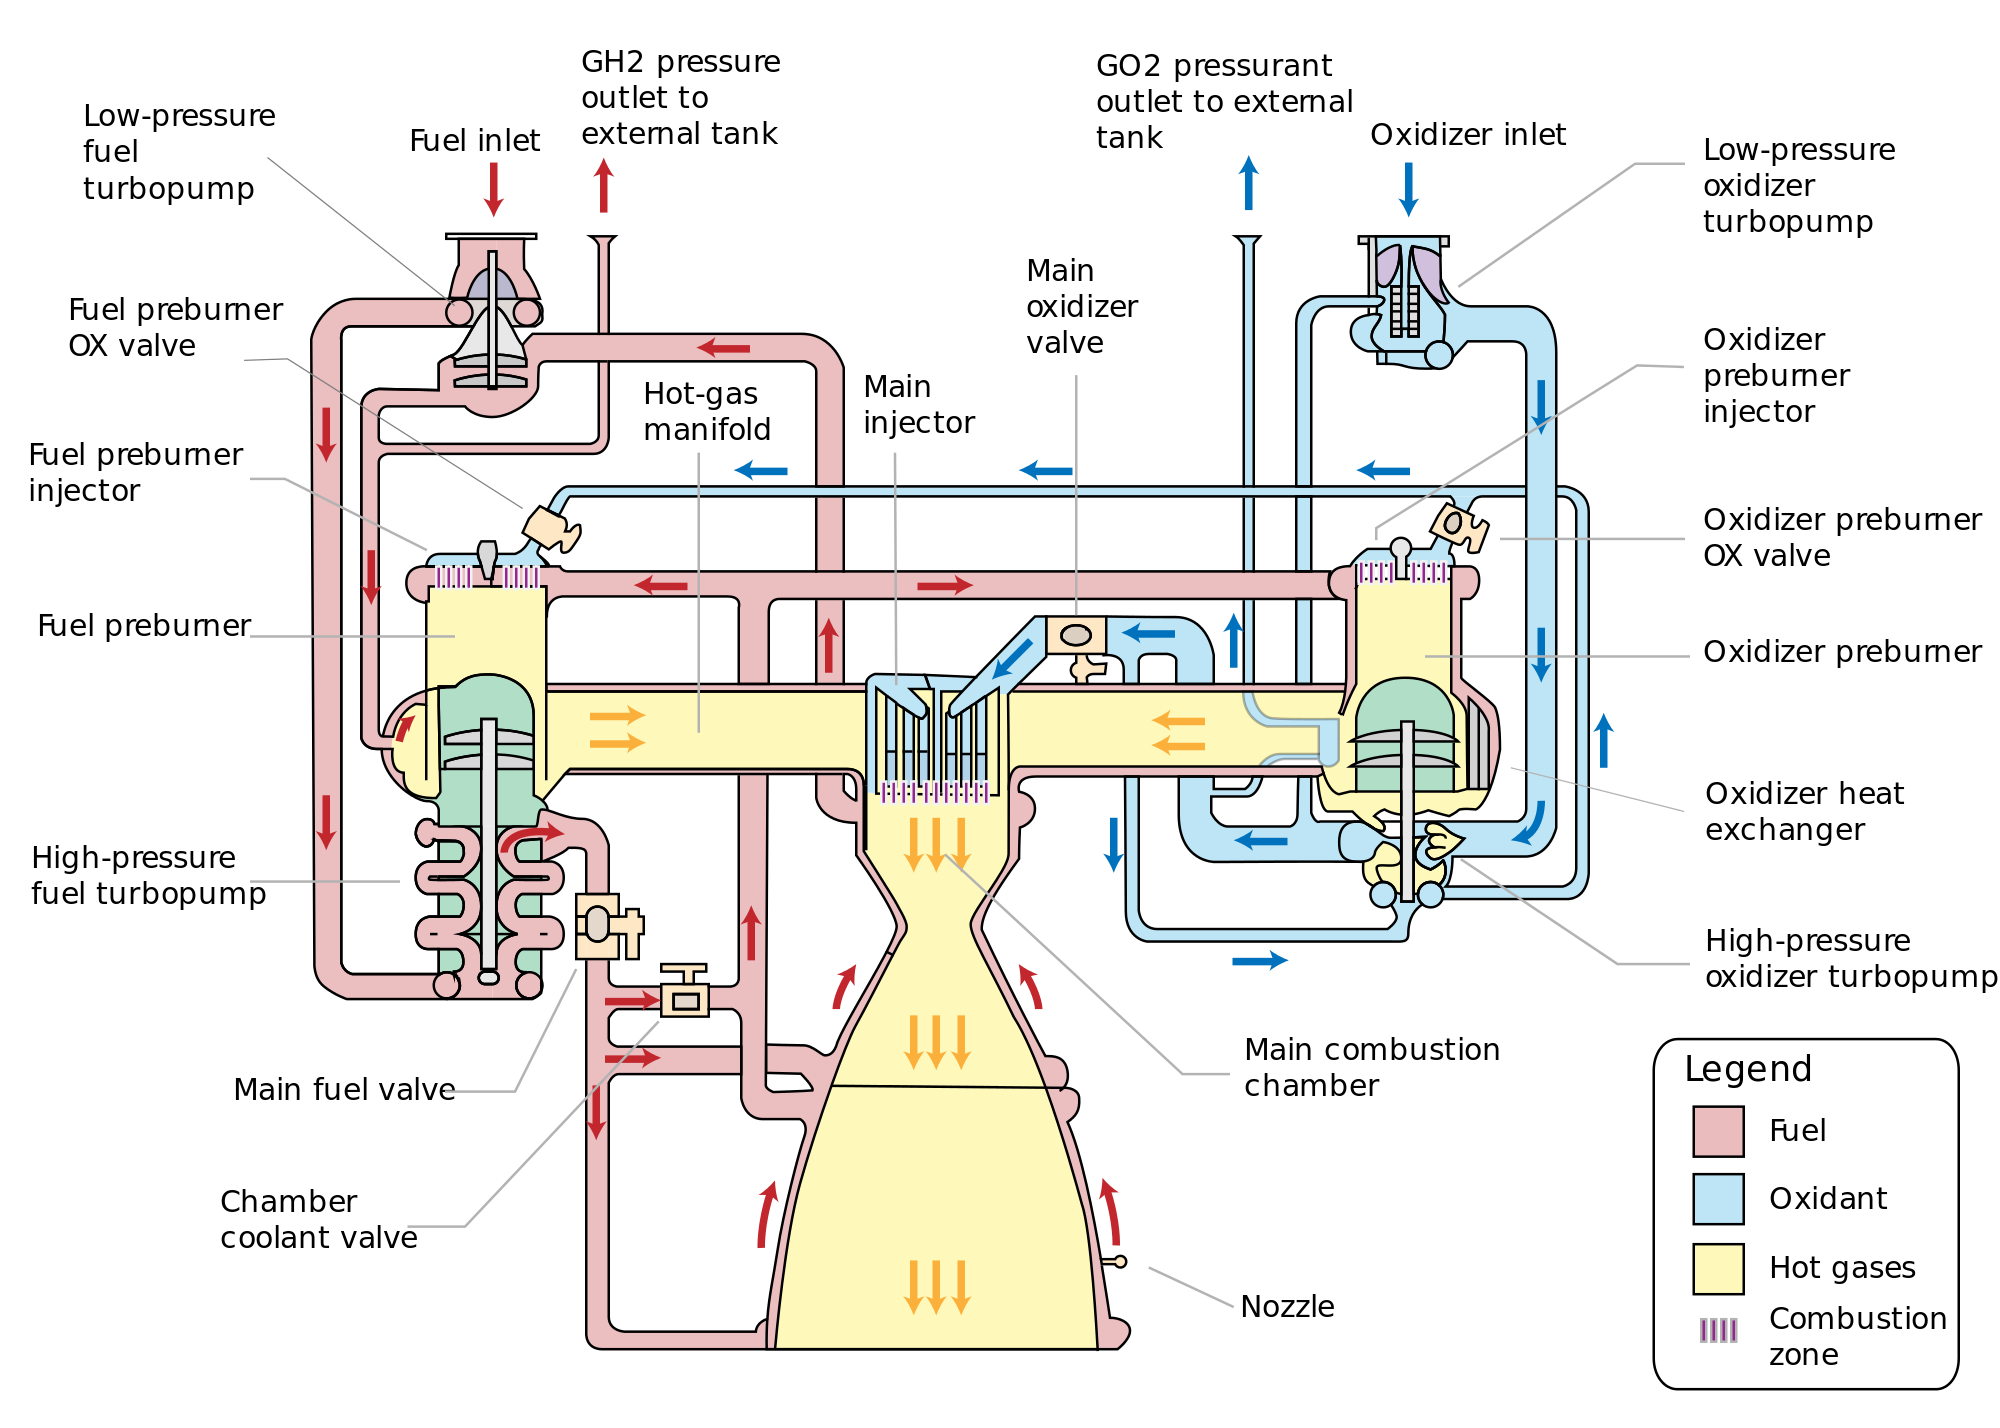
\includegraphics[width=0.6\textheight, angle=0,origin=c]{chapter_1/Ssme_schematic_(updated).svg.png}
    \caption{Умовна схема роботи РРД RS-25 з насосною подачею компонентів палива}
    \label{fig:SSME}
\end{figure}

Компоненти палива --- паливо і окиснювач надходять з баків на відцентрові насоси, що приводяться в рух газовою турбіною. Під високим тиском компоненти палива надходять на форсункову головку  --- вузол, в якому розміщені форсунки, через які компоненти нагнітаються в камеру згоряння, перемішуються і згорають, створюючи нагріте до високої температури газоподібне робоче тіло, яке, розширюючись у соплі, здійснює роботу і перетворює внутрішню енергію газу в кінетичну енергію його направленого руху. Через сопло газ виходить з великою швидкістю, надаючи двигуну реактивну тягу.

Паливна система РРД складається з елементів, що використовуються для подачі палива в камеру згоряння — паливних баків, трубопроводів, турбонасосного агрегату — вузла, що складається з насосів і турбіни, змонтованих на єдиному валу, форсункової голівки і клапанів, які регулюють подачу палива. Насосна подача палива дозволяє створити в камері двигуна високий тиск, від десятків до сотень атмосфер. Високий тиск забезпечує більший ступінь розширення робочого тіла, що є передумовою для досягнення високого значення питомого імпульсу. Крім того, при великому тиску в камері згоряння досягається краще значення тягооснащеності двигуна — відношення величини тяги до маси двигуна. Чим більше значення цього показника, тим менше розміри і маса двигуна (за тієї ж тяги), і тим вище ступінь його досконалості. Переваги насосної системи особливо позначаються в РРД з великою тягою --- наприклад, у рушійних установках ракет-носіїв.

Відпрацьовані гази з турбіни ТНА надходять через форсункову голівку в камеру згоряння разом з компонентами палива. Такий двигун називається двигуном із замкнутим циклом (інакше — з закритим циклом), при якому усе витрачене паливо, включаючи використовуване в приводі ТНА, проходить через камеру згоряння РРД (рис.~\ref{fig:closed_cycle}).

\begin{figure}
    \centering
    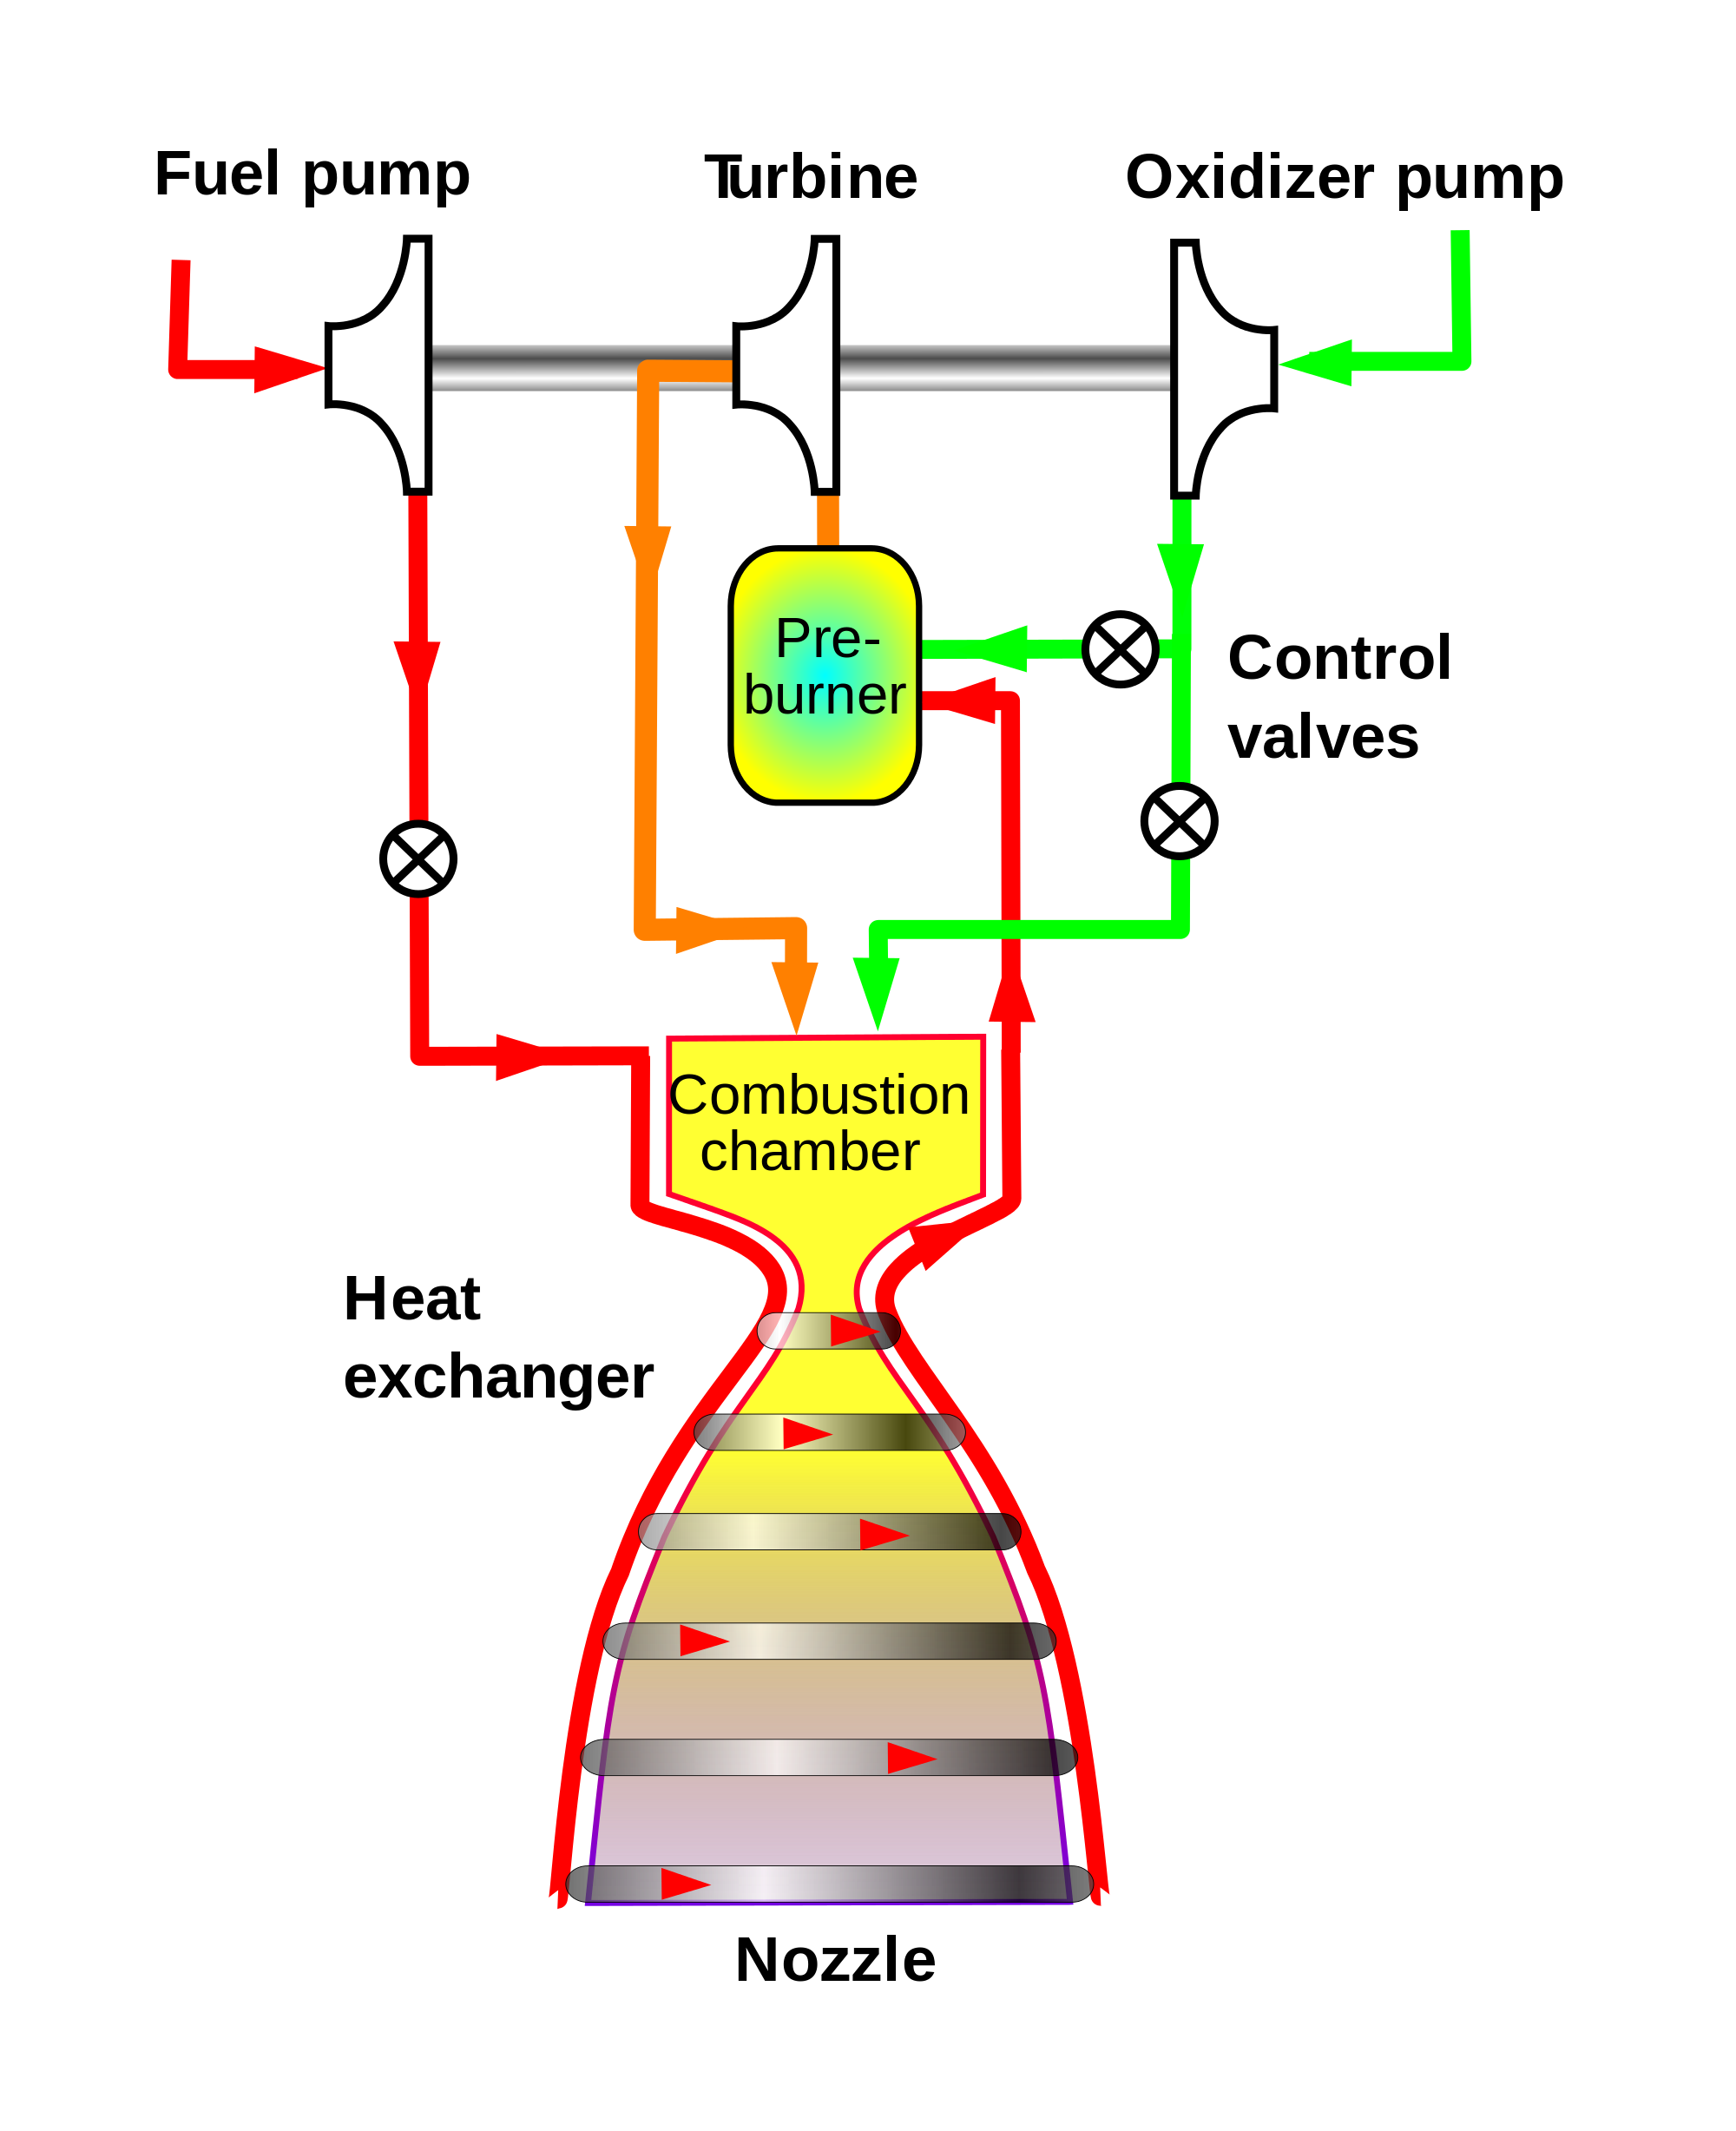
\includegraphics[width=0.35\textheight, angle=0,origin=c]{chapter_1/Staged_combustion_rocket_cycle.svg.png}
    \caption{Принципова схема РРД закритого циклу (англ. closed cycle engine)}
    \label{fig:closed_cycle}
\end{figure}

Тиск на виході турбіни в такому двигуні вищий, ніж у камері згоряння РРД, а на вході в газогенератор, що приводить в рух турбіну, --- ще вище. Щоб задовольнити ці вимоги, для приводу турбіни використовуються ті ж компоненти палива (під високим тиском), на яких працює сам РРД (з іншим співвідношенням компонентів, як правило, -- з надлишком пального, щоб знизити теплове навантаження на турбіну).

Альтернативою замкнутому циклу є відкритий цикл, при якому вихлоп турбіни викидається прямо в навколишнє середовище через відвідний патрубок (рис.~\ref{fig:gas_generator}).

\begin{figure}
    \centering
    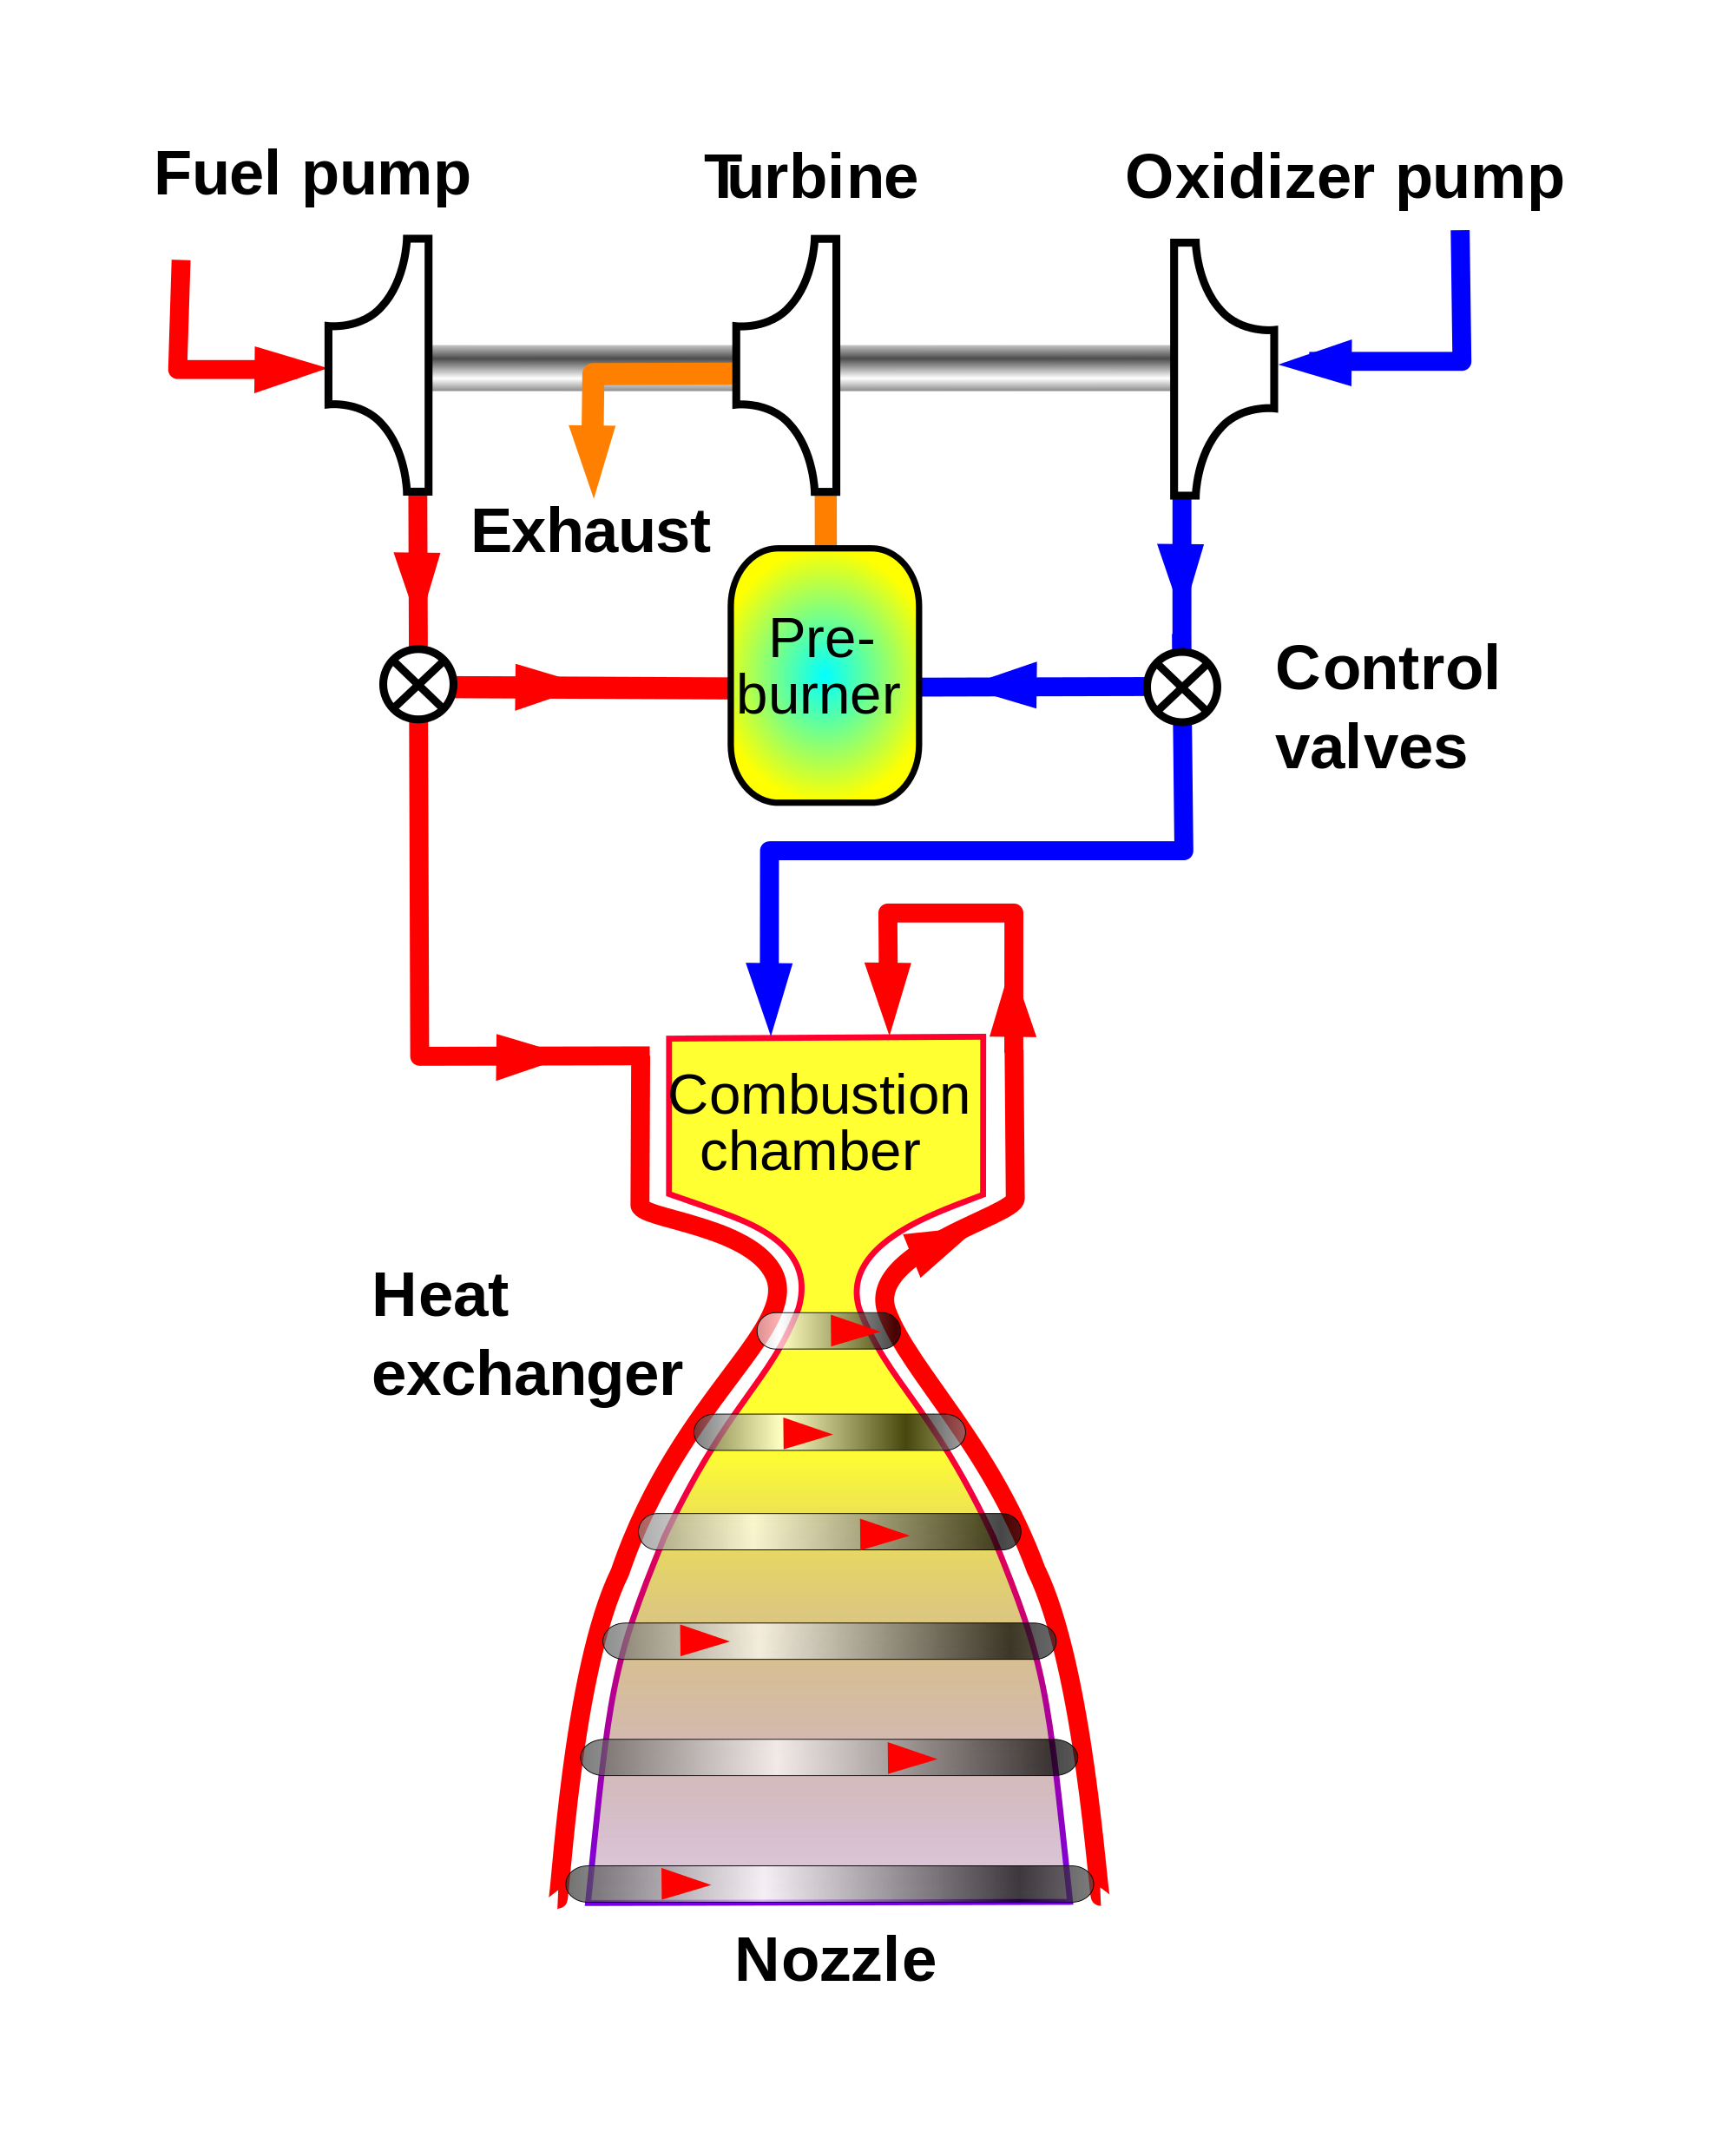
\includegraphics[width=0.35\textheight, angle=0,origin=c]{chapter_1/Gas_generator_rocket_cycle.svg.png}
    \caption{Принципова схема РРД відкритого циклу (англ. gas generator cycle engine)}
    \label{fig:gas_generator}
\end{figure}

Реалізація відкритого циклу технічно простіша, оскільки робота турбіни не пов'язана з роботою камери РРД, і в цьому випадку ТНА взагалі може мати свою незалежну паливну систему, що спрощує процедуру запуску всієї рушійної установки. Але системи з замкнутим циклом мають трохи кращі значення питомого імпульсу, і це змушує конструкторів долати технічні труднощі їхньої реалізації, особливо для великих двигунів ракет-носіїв, до яких пред'являються особливо високі вимоги за цим показником.

При невеликій тязі двигуна (і, отже, невеликій витраті палива) турбонасосний агрегат стає занадто важким елементом, що погіршує масові характеристики рушійної установки. Альтернативою насосній паливній системі служить витискувальна, при якій надходження палива в камеру згоряння забезпечує тиск наддуву в паливних баках, створюваний стисненим газом, найчастіше азотом, який є незаймистим, неотруйним, не є окиснювачем і порівняно дешевий у виробництві (рис.~\ref{fig:pressure_fed}).

\begin{figure}
    \centering
    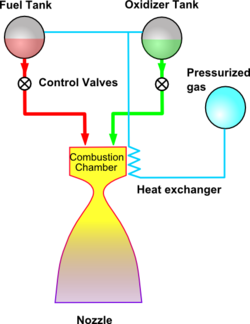
\includegraphics[width=0.4\textheight, angle=0,origin=c]{chapter_1/Pressure_fed_rocket_cycle.png}
    \caption{Принципова схема РРД з витискувальною подачею палива (англ. pressure-fed engine)}
    \label{fig:pressure_fed}
\end{figure}

Для наддуву баків з рідким воднем використовується гелій, оскільки інші гази при температурі рідкого водню конденсуються і перетворюються в рідини~\cite{Dorofeyev}.

Аналогом газогенераторного циклу є інша схема роботи РРД, двигун такої схеми і розглядатиметься  у ході роботи --- цикл з фазовим переходом (англ. expander cycle) (рис.~\ref{fig:expander_cycle}).

\begin{figure}
    \centering
    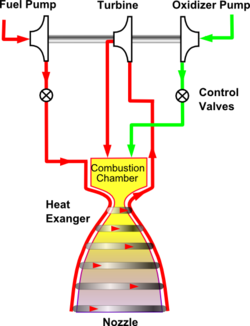
\includegraphics[width=0.4\textheight, angle=0,origin=c]{chapter_1/Expander_rocket_cycle.png}
    \caption{Принципова схема циклу РРД з фазовим переходом (безгазогенераторний РРД) (англ. expander cycle engine)}
    \label{fig:expander_cycle}
\end{figure}

Принцип роботи циклу з фазовим переходом полягає у збільшенні енергії потоку пального (а також окиснювача у деяких варіантах виконання) за рахунок тепла, виділеного камерою згоряння. Тепло передається охолоджуючим кожухом, розташованим навколо КЗ і сопла. Потік, що увібрав теплоту, направляється у ТНА, який відбирає частину енергії потоку для розкрутки турбін пального і окиснювача. Щойно випущений з ТНА потік впорскується в КЗ і згоряє у випадку закритого циклу з фазовим переходом, або ж викидається з контура у варіанті відкритого циклу. Зазвичай у таких установках використовуються кріогенні паливні компоненти, наприклад рідкі водень (\ce{LH2}) та кисень (\ce{LOX}).

Функція турбонасоса у такому циклі полягає у збільшенні тиску у потоці до значення, що компенсує перепад тиску в системі охолодження та контурі загалом, спад тиску внаслідок розширення у турбіні та забезпечує необхідний тиск у форсуночній камері. 

Надійність установок, що використовують цикл з фазовим переходом, забезпечується простотою схеми і відносно малими механічними й тепловими навантаженнями на переріз турбіни. Межа використання такого циклу двигуна пов'язана із значенням температури на вході в турбіну, оскільки площа, яку покриває охолоджувальний кожух, обмежена. Проблема пояснюється законом квадрата-куба: зі зростанням розмірів сопла внаслідок збільшення тяги, площа його поверхні збільшується пропорційно квадрату діаметра, проте об'єм пального, що потрібно нагріти, зростає пропорційно діаметру в кубі. Звідси маємо, що існують максимальні габарити двигуна, поза якими площі поверхні сопла вже не вистачає для нагрівання пального, достатнього для розкрутки ним турбіни і відповідно усього ТНА~\cite[с. 5 -- 6]{Cantiani}.


\section{Процеси, протікаючі в камері згоряння РРД}

Рідинний ракетний двигун є складним пристроєм, у камері згоряння якого протікає не лише екзотермічна реакція окиснення пального, а й низка важливих супутніх явищ, що є взаємопов'язаними: зокрема це газодинамічне прискорення робочого тіла через перепад тисків на вході й виході та його ізобарне нагрівання.

\subsection{Хімічна кінетика: горіння в КЗ}

У типовому рідинному ракетному двигуні тиск всередині камери згоряння може досягати 200 атмосфер, що є набагато більшим, ніж тиск в інших більш поширених двигунах внутрішнього згоряння, таких як автомобільний чи газотурбінний. Для того, щоб зрозуміти та спрогнозувати процес горіння у РРД, потрібен новий деталізований кінетичний механізм системи \ce{H2 / O2}, оскільки усі моделі, запропоновані до цього часу, не були перевіреними за умов високого тиску, що обмежує їх застосування. Збір експериментальних даних для отримання констант швидкості реакції за таких складних умов сам по собі є задачею, вартою окремого фізико --- хімічного дослідження. Деякі константи можуть бути розраховані теоретично, без використання результатів експерименту. Окрім того, у горінні палива в РРД не задіяний розчинник, водночас в багатьох експериментальних установках для визначення швидкості горіння полум'я чи затримки займання присутні азот чи аргон. Це також ускладнює задачу створення детальної кінетичної моделі, що може описувати процеси в РРД.~\cite[с. 383 -- 384]{Shimizu}

У табл.~\ref{chem_kin_h2} наведена детальна кінетична модель, що в рамках даного дослідження~\cite{Shimizu} включає в себе більшість відомих елементарних реакцій між сполуками та радикалами \ce{H2}, \ce{O2}, \ce{H2O}, \ce{H}, \ce{O}, \ce{OH}, \ce{HO2}, і \ce{H2O2}. Дана модель створювалась із використанням уточнених або перерахованих констант реакцій розроблених у попередній моделі авторства Кітано та ін.~\cite[с. 2355 -- 2362]{Kitano}. У процесі розробки цієї моделі не передбачалось узгодження констант реакцій з перевірочними даними, окрім випадку з \ce{H + OH + M = H_2O + M}. Натомість, ці значення брались з надійних літературних джерел. У першу чергу потрібно було визначити величину показників трикомпонентних взаємодій (англ. third-body efficiencies --- авт.) для \ce{H2}, \ce{O2} і \ce{H2O}, оскільки вони є важливими у рамках моделі та впливають на її точність в умовах високого тиску та відсутності розчинника.~\cite[с. 384 -- 385]{Shimizu}.

Для отримання валідних і верифіковних результатів термодинамічних розрахунків камери гібридної електрохімічної ракетної установки необхідно враховувати кінетику хімічних реакцій компонентів паливної суміші за умов високих температур і тисків РРД у присутності частинок присадки, що може призвести до інтенсифікації або сповільнення цих реакцій у камері згоряння (КЗ) двигуна. Високотемпературні реакції за високих тисків, характерних для РРД, ретельно досліджувались та описані у роботах багатьох авторів, зокрема~\cite{Shimizu} для воднево-кисневої суміші. На практиці для опису таких процесів у галузі застосовуються спеціальні програмні пакети, що враховують особливості термодинаміки КЗ ракетних двигунів. Одним із таких є \texttt{Астра.4/рс}, що дозволяє моделювати дво- і трикомпонентні реакції горіння за визначеними моделями таких процесів при заданому тиску (процеси у камері за визначенням циклу Брайтона ізобарні) та співвідношенні компонентів~\cite{Astra}. Пакет написаний мовою \texttt{Fortran}, для роботи застосовується оболонка у середовищі \texttt{Python}. 


\subsection{Термодинамічний опис}

Камера згоряння (КЗ) --- це частина РД, де відбувається власне процес горіння паливної суміші. Температура горіння палива чи не завжди є більшою, ніж температура плавлення матеріалів стінок камери. Отже, основними проблемами цієї частини двигуна є охолодження та/або обмеження часу роботи окремих вузлів під тепловим навантаженням.

Найчастіше камери згоряння виконуються циліндричної форми, з подальшим звуженням до критичного перерізу сопла уздовж осі симетрії. Форма й об'єм КЗ обираються відповідно до основних керуючих параметрів: необхідного значення об'єму для повного змішування і згоряння паливної суміші, спаду тиску газу уздовж осі для прискорення РТ (має бути мінімальним для мінімізації спаду швидкості витікання, а отже й тяги та питомого імпульсу), величини критичного перерізу, що визначає тиск у камері та відповідно її допустимі габарити за даних характеристик і матеріалів тощо.

Теплота передається до усіх внутрішніх поверхонь та обладнання, що відкриті до потоку розжарених газів, зокрема на плиту інжектора, стінки камери і сопла. Густина теплового потоку у камері залежить від параметрів конкретного двигуна; в основному лише  $0.5\ldots 5$~\% усієї енергії, вивільненої газом, передається у вигляді теплоти на стінки камери. Для типового двигуна тягою 44820 Н (10000 lbf) тепловий потік на стінку КЗ може сягати $0.75 -  3.5$~МВт, в залежності від фактичних умов роботи  й конструкції.

Кількість теплоти, що передається через теплопровідність газу камері є нехтуваною. Найбільшим за часткою є конвективний теплообмін. Частину (зазвичай від 5 до 35\%) становить радіаційна передача теплоти.

За фіксованого параметру тиску у КЗ та збільшенні тяги двигуна площа поверхні зростає менш швидко, ніж об'єм. Тому охолодження камери легше реалізується у великих габаритах установки, водночас у менших двигунах знятий системою охолодження тепловий потік є критично важливим параметром внаслідок дії закону квадрата-куба.

Вищий тиск у камері згоряння спричиняє збільшення питомого імпульсу, поряд з тим збільшуючи масу двигуна. Однак, результуюче збільшення інтенсивності теплообміну зі стінкою часто накладає межі зростання практичного значення тиску у КЗ як для твердопаливних, так і для рідинних РД.

Величина теплового потоку у хімічних РД може варіюватись від менш, ніж $50~W/cm^{2}$ до понад $16~kW/cm^{2}$. Найбільшими є значення у критичному перерізі великогабаритних КЗ та твердопаливних РД високого тиску. Меншими є показники для газогенераторів, ділянок біля зрізу сопла, або малих КЗ малого тиску~\cite[с. 282 -- 286]{Sutton}.

\subsection{Газодинамічні процеси}

У типовому надзвуковому соплі велика частина теплової енергії газу в КЗ перетворюється у кінетичну енергію його руху. Тиск газу і його температура швидко спадають, водночас швидкість може досягати кількох миль за секунду. Це зазвичай є ізоентропійним процесом. Якщо внутрішня стінка сопла має дефект (зварний шов чи скол), кінетична енергія газу локально перетворюється у теплову, причому температура й тиск приймають значення таких для потоку газу у камері, спричиняючи руйнування стінки; отже, вона має бути гладкою і позбавленою нерівностей.

Температура у КЗ в ізоентропійному процесі мало відрізняється від стагнаційної температури (температури горіння у хімічних РД). Швидкість витікання газу з сопла є функцією відношення тисків у КЗ і ззовні, адіабатичного показника продуктів згоряння, а також температури на вході у сопло і газової сталої для даної суміші. Оскільки газова стала пропорційна молярній масі, швидкість витікання (або ж питомий імпульс, має розмірність швидкості) є функцією відношення температури на вході у сопло і молярної маси потоку. Це відношення є важливим для оптимізації масової пропорції компонентів палива.

Максимальна теоретична швидкість витікання є скінченною, попри те, що відношення тисків може бути нескінченно великим; це пов'язано з тим, що внутрішня енергія хімічних сполук приймає скінченне значення; нескінченного розширення відбутись не може, оскільки воно призводить до фазових переходів газу.

У соплах ракетних двигунів можуть бути отримані великі швидкості витікання (більші, ніж  $1$~км/с). Спад температури продуктів згоряння є дуже помітним; уздовж короткого відрізку вона може падати на  $2-3$ порядки. Зі збільшенням кінетичної енергії руху потоку газу зменшується його ентальпія, що пропорційно знижує температуру. Оскільки газ одразу після проходження зрізу сопла усе ще є розжареним (типові температури порядку $1000$ К), він містить істотну кількість тепла, не перетвореного у кінетичну енергію потоку.

Неідеальна поведінка камер і сопел РД тісно пов'язана з присутністю у реальних установках стрибків ущільнення, або ж ударних хвиль, що здебільшого виникають у дифузорній ділянці сопла й існують лише у надзвукових потоках. Хвилі розрідження, що також є суто надзвуковим феноменом, утворюються за зрізом сопла й знижують тиск потоку до значень, відповідних навколишньому середовищу.~\cite[с. 52 -- 69]{Sutton}

\section{МПД-прискорювач: узагальнений опис пристрою}

\begin{figure}
	\centering
	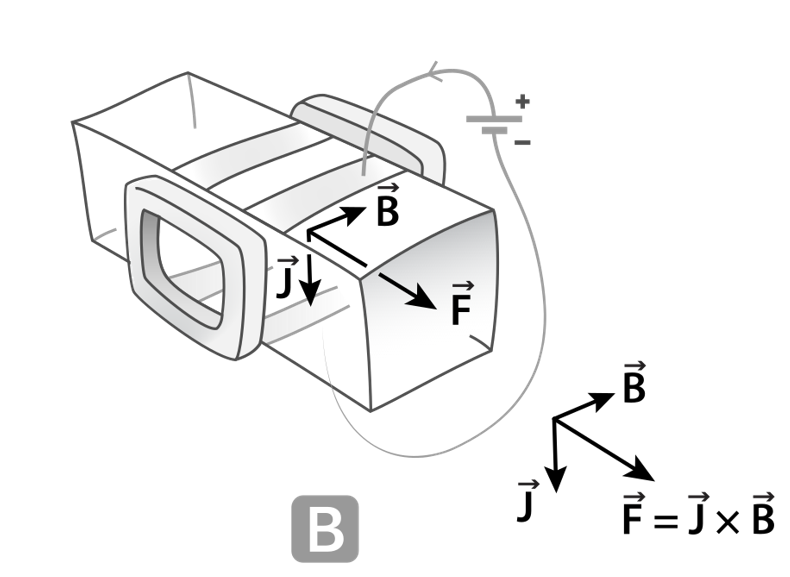
\includegraphics[width=0.6\textheight, angle=0,origin=c]{chapter_1/MHD_thruster_principle.png}
	\caption{Ілюстрація принципу роботи МПД-прискорювача}
	\label{fig:MHD_thruster_principle}
\end{figure}

\begin{figure}
	\centering
	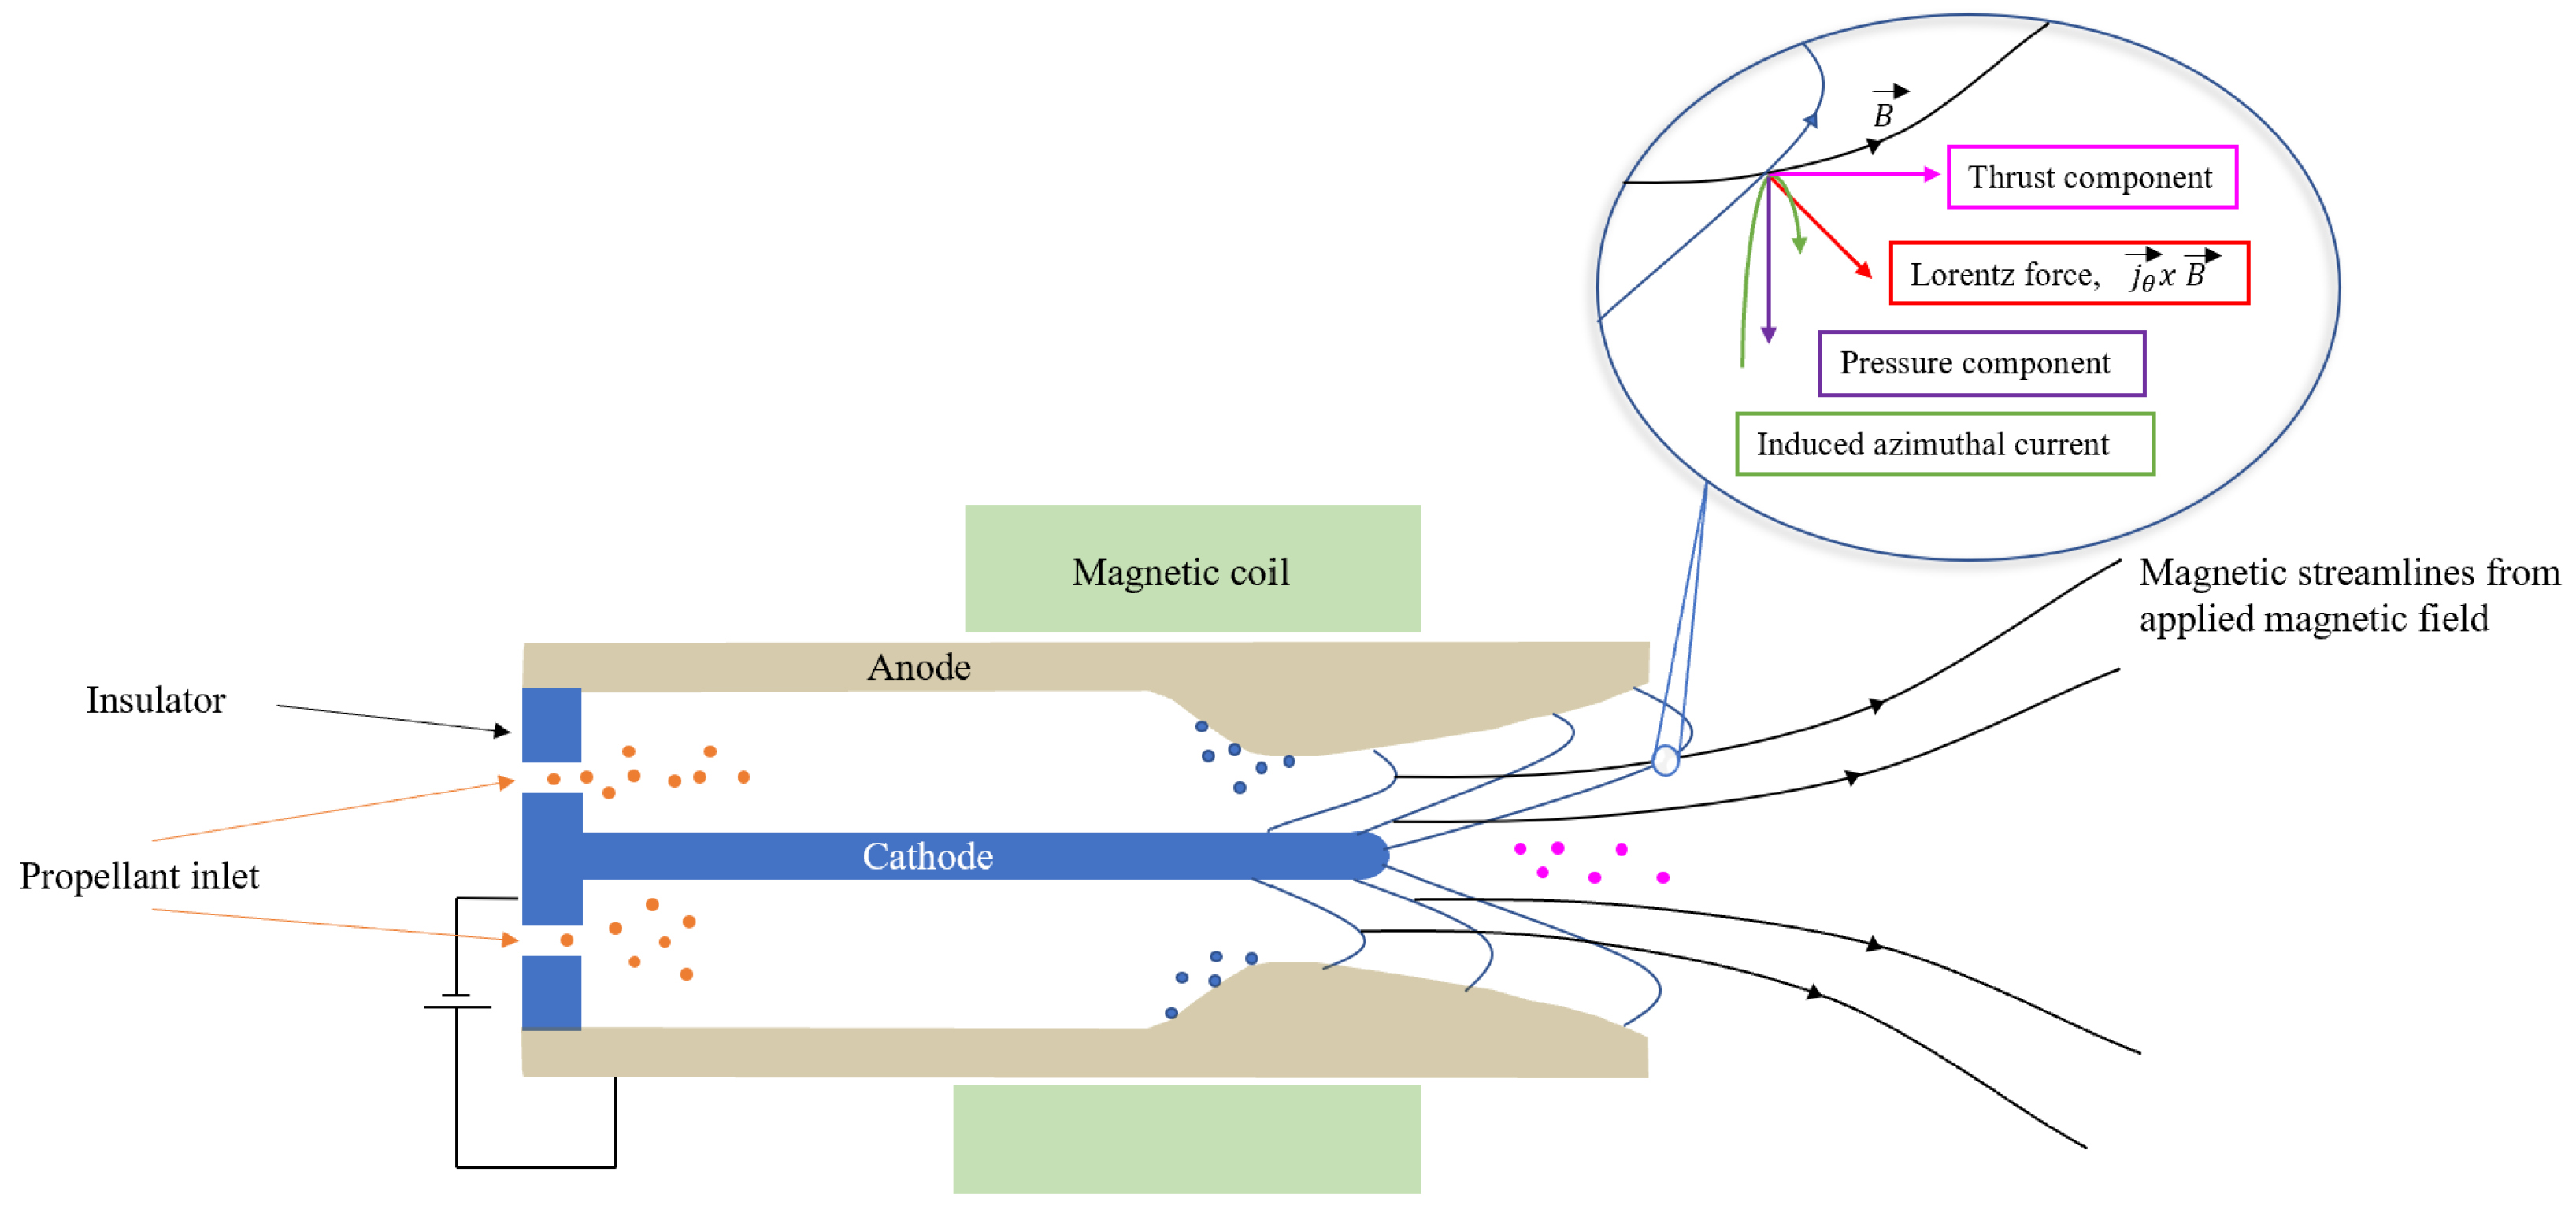
\includegraphics[width=0.6\textheight, angle=0,origin=c]{chapter_1/MHD_thruster_coaxial.jpg}
	\caption{Схема роботи МГД-прискорювача (аналог; катод показаний коаксіальним)}
	\label{fig:MHD_thruster_coaxial}
\end{figure}

Для надання кінетичної енергії потоку робочого тіла (порошок присадки металічного калію, що іонізується у потоці розжареного газу РРД) МПД-прискорювач використовує схрещені електричне та магнітне поля, що створюються протилежно розташованими електродами і котушками з віссю, перпендикулярною до осі каналу, по якому рухається робоче тіло (МПД-канал, він же у плазморідинному двигуні є камерою і соплом РРД) (рис.~\ref{fig:MHD_thruster_principle}). Принципова схема рушійної МГД-установки наведена на рис.~\ref{fig:MHD_thruster_coaxial}; на схемі один з електродів розташований коаксіально, у схемі ж плазморідинного двигуна, що розглядається, обидва електроди розміщені на протилежних стінках МПД-каналу.

В МГД-прискорювачах щільних плазмових середовищ проходить зворотнє до МГД-генератора перетворення виду енергії, тобто електрична енергія, яку ми підводимо, перетворюється в кінетичну і теплову. В каналі МГД-прискорювача відбувається прискорення плазмового середовища під дією пондеромоторної сили (сили Ампера), що дозволяє отримати в лабораторних умовах гіперзвукові швидкості потоку, характерні для аерокосмічних польотів. При швидкостях повітряного чи газового потоку з числом Маха $M > 10$ температура, ентальпія і гальмівний тиск досягають величин, неможливих при спаленні хімічного палива ($> 10$~кК, $>20$~МДж/кг, $\ge 1000$ ат відповідно). МГД-прискорювачі вже знайшли практичне використання у складі аеродинамічних труб для моделювання аерокосмічних польотів та високошвидкісного обтікання тіл (конструкцій).~\cite[с. 10]{Panchenko}

\section{Бар'єр питомого імпульсу існуючих РД}

Основні параметри ракетних двигунів (тяга та питомий імпульс) мають обмеження, пов'язані здебільшого з умовами протікання процесів надання енергії робочому тілу.

Усі розглянуті схеми РРД у більшій чи меншій мірі розв'язують одну й ту ж проблему --- збільшення питомого імпульсу за умови збереження тягооснащеності (додавання газогенератора, замикання контуру пального та окиснювача на камері згоряння тощо); це зводиться до простого підвищення тиску в КЗ, а він у свою чергу залежить від теплоти згоряння пального та тиску в системі перед КЗ, що пов'язані з потужністю ТНА пального та окиснювача; відповідно маємо, що ефективність РРД обмежена максимальною теплотою згоряння в КЗ, або ж у випадку використання газогенератора --- температурою плавлення лопаток його турбіни. Ці параметри зумовлюють обмеження питомого імпульсу двокомпонентних РРД величиною близько $4800$ м/с (близько $490$~с); в істотно важчих з точки зору технічної реалізації трикомпонентних схем рекордне значення досягає $542$ с (паливна суміш літій -- водень -- фтор). 

Виникає потреба усунути або ж компенсувати обмеження швидкості РТ, надавши йому додаткову енергію. Відомо, що за тисків та температур у КЗ набуває істотності процес дисоціації продуктів згоряння та їх часткової іонізації. Ступінь іонізації газу є незначним (близько 1-2 процентів), проте надалі надавати теплоту робочому тілу невигідно, оскільки основний механізм її надання (горіння) переривається внаслідок вищезгаданої рекомбінації реагентів. Поряд із цим надлишкова енергія РТ, що частково йде на іонізацію, у РРД ніяк не використовується. Газодинамічна складова проблеми полягає у неможливості адаптації сопла до широкого діапазону навколишніх тисків; за надто високих значень тиску середовища має місце перерозширення сопла, за малих --- недорозширення; використання соплових насадків є невигідним через відсутність можливості плавної адаптації РД до зміни тиску.

МПД-установки були апробовані в якості двигунів малої тяги для супутників, проте для їх роботи потрібне потужне джерело електроенергії, що зменшує тягооснащеність силової установки до значень, неприйнятних для використання в ролі маршової рушійної установки в межах атмосфери; ця ж проблема постає для всіх існуючих електричних ракетних двигунів.

%Сучасні розроблені ядерні ракетні двигуни, що мають теоретично достатнє для атмосферного використання значення тягооснащеності, діють за принципом реакторних установок з протікаючим крізь активну зону робочим тілом; відповідно РТ такого двигуна є радіоактивним, це зумовлює неможливість його використання в межах атмосфери Землі. Інші схеми роботи ЯРД (рідинно- та газофазні типу "ядерної лампи"), що не передбачають прямого контакту РТ з активною зоною реактора, не можуть бути реалізовані з використанням існуючих матеріалів та технологій.

\section{Плазморідинний ракетний двигун: проблематика і принцип роботи}

Новий тип ракетного двигуна, принцип роботи якого теоретично та чисельно описується у цій роботі, є потенційно ефективнішим, ніж існуючі зразки рідинних ракетних двигунів, і відповідно виступає кращим зразком рушійної установки для верхніх ступеней ракет-носіїв для виведення вантажів по траєкторії з верхніх шарів атмосфери у вакуум на низькі й перехідні орбіти Землі з меншими втратами палива і питомого імпульсу --- це рідинний ракетний двигун з магнітоплазмодинамічним прискорювачем, або плазморідинний ракетний двигун.

Така установка може вирішити проблему ефективного високоатмосферного РД шляхом комбінування РРД та МПД-прискорювача в гібридну установку, що використовує як хімічний/газодинамічний, так і електромагнітний способи надання енергії РТ для збільшення швидкості витікання, а отже і питомого імпульсу.

Рідинні ракетні двигуни мають дуже велику кількість різновидів конструкцій та схем роботи: двигуни з витіснювальною подачею палива, турбонасосні відкритого циклу, закритого циклу з допалюванням окиснювального, генераторного газу тощо~\cite{Dobrovolskiy}. Розглядаючи новий тип гібридного двигуна, варто обирати тип РРД, що відповідає двом показникам: 
\begin{itemize}
	\item якомога більший питомий імпульс;
	\item можливість використання потужності двигуна для живлення МПД-прискорювача.
\end{itemize}


Такими різновидами РРД є безгенераторні двигуни з фазовим переходом (англ. \texttt{expander cycle engine}) та двигуни закритого циклу~\cite{Sutton}. Перші відрізняються відсутністю газогенератора, що полегшує та спрощує конструкцію двигуна, проте позбавляють можливості масштабування через те, що потужність установки обмежується властивостями робочого тіла (палива) --- у безгенераторних двигунів зазвичай використовується водень як пальне з найбільшим відношенням внутрішньої енергії до молярної маси, проте теоретична потужність такого двигуна незначна. Можливість зняття потужності з безгенераторного двигуна відсутня, оскільки уся енергія робочого тіла використовується для розкрутки турбонасосного агрегата (ТНА). 
Двигуни закритого циклу можуть мати значну тягу та питомий імпульс --- їхні характеристики обмежуються допустимим тиском у газогенераторі, що використовується для розкрутки ТНА і має бути більшим за тиск у камері згоряння~\cite{Ovsyannikov}. Проте уся енергія робочого тіла такого РРД використовується для максимізації потужності насосів та збільшення тиску у камері згоряння, що виключає можливість відбору потужності з установки без істотних змін у конструкції газогенератора і турбіни.

Отже, для інтеґрації РРД і МПД-прискорювача без додавання окремої енергоустановки, використовуючи внутрішню енергію палива РРД, необхідно використати цикл і принципову схему двигуна, що передбачатиме наявність окремої газової турбіни, не пов'язаної з ТНА РРД принаймні на його номінальному режимі.

Електромагнітне прискорення РТ вимагає певних значень ступеня його іонізації; продукти згоряння РРД мають високу температуру та достатньо надлишкової енергії через високий тиск у КЗ, проте іонізованих частинок там недостатньо. Для збільшення ступеня іонізації потоку в нього через окрему форсунку на етапі змішування вводиться присадка дрібнодиспергованого калію у розмірі декількох процентів від масової витрати двигуна; калій обраний через його малу енергію іонізації, що зумовлює найбільш повний перехід у потік заряджених частинок, що можуть бути прискорені електромагнітним полем МПД-каналу; у моделях, що розглядаються у розділі~\ref{sec:model_conditions}, вхідний переріз потоку з паливом РРД спільний. МПД-канал згідно такої схеми подачі присадки розташовується у закритичному перерізі сопла РРД, що є принциповою відмінністю поряд із конструкціями, що розглядались у попередніх роботах~\cite{Previous}.


\section{Висновки до розділу \ref{sec:First}}

Проведений аналіз літературних джерел показав, що рідинні ракетні двигуни мають межу ефективності, пов'язаний з бар'єром питомого імпульсу цих установок --- кінетична енергія руху обмежується внутрішньою енергією паливних компонентів, а зовнішнє підведення енергії відсутнє, що призводить до зменшення ефективності використання літальних апаратів з цими двигунами.

Запропонована принципова схема плазморідинного ракетного двигуна потребує належного числового моделювання термодинаміки процесів у ньому, для подальшої валідної оцінки її ефективності, потребується змоделювати термо- та газодинаміку потоку робочого тіла РРД і МПД-прискорювача у спільному середовищі. Також необхідно враховувати конструктивні обмеження конфігурації гібридної рушійної установки внаслідок особливостей умов роботи МПД-компонента.

З урахуванням особливостей процесів, розглянутих під час аналізу літературних джерел, результати числового моделювання ТД-процесів у РРД за присутності робочого тіла МПД-установки дозволять кількісно оцінити ефективність поєднання РРД і МПД-прискорювача у межах однієї рушійної установки. 
\chapter{Моделювання термодинамічних процесів у камері. Оцінка параметрів МПД-прискорювача}\label{sec:model_conditions}

\section{Числова модель ТД-розрахунків: комплекс Астра.4}


В основу алгоритму багатоцільовоого програмного комплексу \texttt{Астра.4/рс} покладений універсальний термодинамічний метод визначення характеристик довільних гетерогенних систем, заснований на фундаментальному принципі максимуму ентропії. Цей метод надає можливість узагальненого опису будь-якого високотемпературного стану за допомогою фундаментальних законів термодинаміки, незалежно від умов та способів досягнення стану рівноваги. Метод потребує мінімальної інформації про саму систему та її оточення.

Формулювання задачі ТД-моделювання полягає у призначенні двох умов рівноваги досліджуваної системи з навколишнім середовищем. Ними можуть бути або числові значення ТД-характеристик, або функціональні співвідношення між ними.

Допущення моделі розрахунку у комплексі наступні:
\begin{itemize}
	\item розглядаються системи у стані зовнішньої та внутрішньої термодинамічної рівноваги (повної чи локальної);
	\item розглядаються замкнені системи, тобто такі, що не обмінюються речовиною з навколишнім середовищем;
	\item присутність газової фази є обов'язковим; газова фаза описується рівнянням стану ідеального газу;
	\item поверхневі ефекти на границі поділу фаз не враховуються, розчинність газів у рідкій та твердій фазі відсутня;
	\item конденсовані речовини утворюють однокомпонентні незмішувані фази, або включаються у склад ідеальних конденсованих розчинів.
\end{itemize}

Допускається наявність інших параметрів:
\begin{itemize}
	\item виключення зі складу враховуваних компонентів рівноваги будь-яких індивідуальних речовин;
	\item можливість призначати (фіксувати) концентрації однієї або декількох речовин з подальшим розрахунком рівноваги іншої частини системи;
	\item розгляд неідеальних конденсованих розчинів шляхом введення надлишкової енергії Гіббса;
	\item врахування власного об'єму, що займають конденсовані речовини.	
\end{itemize}

Розрахунки складу фаз та характеристик рівноваги проводяться з використанням внутрішньої бази даних властивостей індивідуальних речовин. База даних є складовою частиною програмного комплексу \texttt{Астра.4/рс}.

Основу інформації у базі даних становлять термодинамічні, теплофізичні та термохімічні властивості індивідуальних речовин, систематизовані у Національному інституті стандартів і технологій США (NIST) та інших ресурсах, опублікованих у відкритих джерелах, обробених розробником комплексу, у тому числі за власними калориметричними та спектроскопічними даними.

У програмному комплексі передбачена можливість введення вихідного складу ТД-систем, утворених дво- та трикомпонентними паливними сумішами за допомогою коефіцієнту надлишку окиснювача та масових часток відповідно. Теоретично необхідне співвідношення компонентів палива, відносно якого задається надлишок окиснювача, обчислюється за допомогою вищих валентностей елементів, що відповідає утворенню повних продуктів згоряння. 

В основному режимі розрахунку параметрів адіабатичного розширення передбачається використання гіпотези локальної термодинамічної рівноваги. Однак можливе проведення обчислень за допомогою різних схем ''заморожування'' складу суміші у соплі.

Програмний комплекс дозволяє виконувати розрахунок ''замороженого'' розширення до заданого тиску, заданого відносного діаметру або ж заданого геометричного ступеня розширення сопла~\cite{Astra}.

Під час розрахунку коефіцієнти втрат питомого імпульсу, втрат в об'ємі камери та соплі для спрощення розрахунку вважались рівними одиниці (розглядається теоретичний випадок поза уточненими експериментально параметрами окремих установок, що можуть індивідуально впливати на ефективність конкретного двигуна).

Процеси впливу електромагнітного поля на потоки іонізуючої присадки та розжарених продуктів згоряння РРД у рамках числової моделі не розглядаються; параметри МПД-прискорювача є результатом оцінки, наведеної у розділі~\ref{sec:model_results}. 

%Модель описує поведінку потоку робочого тіла РРД, враховуючи класичні для такої числової задачі допущення: відсутність в'язкого тертя шарів газу, рух уздовж однієї координатної осі (у нашому випадку вісь абсцис), стисливість за законом ідеального газу (стосується лише взаємодії між частинками самого газу), лагранжева модель дискретної фази для опису руху потоку частинок присадки (металічний дрібнодисперсний калій заданих фракцій з рівномірним розподілом). Задача стаціонарна (програмно використовується опція квазистаціонарності для уточнення розв'язку стаціонарної задачі).

\section{Верифікація моделі. Порівняння з попередніми аналогами}

Для верифікації моделі використовувались технічні параметри існуючого рідинного ракетного двигуна із циклом фазового переходу (expander cycle engine) --- Vinci, що був розроблений у лабораторії DLR Європейського космічного агентства і є одним з найефективніших РРД за показником питомого імпульсу у даний момент~\cite{VinciData}.

У ході попередніх досліджень~\cite{Previous} для побудови аналогічної моделі поведінки потоку робочого тіла у двигуні застосовувався програмний пакет \texttt{ANSYS} Student 2021R1 (підпроцесор Fluent), результати роботи якої було порівняно з розрахунком у пакеті \texttt{Астра.4/рс}.

Основні параметри моделі-аналога:

\begin{itemize}
	\item тип розрахункової моделі - PBСS (Pressure-based Coupled Solver);
	\item чисельно розв'язувалась система рівнянь Ейлера для стисливого газу (нерозривності, збереження імпульсу та збереження енергії)~\cite{GuidePBCS};
	\item задача симетрична відносно осі камери і сопла, була задана кінетична схема горіння пального в окиснювачі (водень/кисень);
	\item модель турбулентності $k-\varepsilon$ з розрахунком релаксаційного множника для турбулентної в'язкості (т. зв. схема Realizable $k-\varepsilon$)~\cite{GuideKEpsilon} із застосуванням методу Finite-Rate/Eddy-Dissipation для уточнення впливу турбулентних течій на кінетику реакцій у КЗ~\cite{GuideChemistry};
	\item застосована радіаційна модель Rosseland із заданим параметром матеріалу стінки та її товщиною~\cite{GuideRosseland};
	\item для моделювання руху частинок присадки застосовується лагранжева модель дискретної фази (DPM) з урахуванням теплообміну між газом та частинками~\cite{GuideDPM}.
\end{itemize}

Граничні умови задані на вході у камеру згоряння (масова витрата палива, а також температура подачі компонентів, зазначена у документації~\cite{VinciDataDLR} - 250 K) і на виході з розрахункової області, зовнішній тиск відповідно до середовища роботи даного РРД становить $50$~мбар ($5$~кПа), температура 293~K.

Товщина стінки камери й сопла - $20$~мм. Матеріал --- алюміній, наявний у переліку матеріалів солвера, коефіцієнти поглинання задані за умовчанням.

Додатково у попередній CFD-моделі було проведене моделювання за присутності присадки калію для визначення оптимального розміру частинок за визначеної масової частки у робочому тілі двигуна.

Умови для потоку присадки - металічний дрібнодисперсний калій з заданими значеннями густини $ 856 $~кг/м$^3$ і теплоємності $871$~Дж/(кг $\cdot$ К); подача присадки здійснюється з входу в камеру згоряння поряд з паливними компонентами, температура 300 K, швидкість подачі взята аналогічною швидкості потоку палива на вході ($118$ м/с ; розраховується автоматично процесором після задання граничних параметрів). Задана витрата становить 0.397 кг/с, що становить 0.01 витрати робочого тіла установки (характерне значення, використовуване в МПД-прискорювачах, згідно даних~\cite{Panchenko}).

\begin{figure}
	\centering
	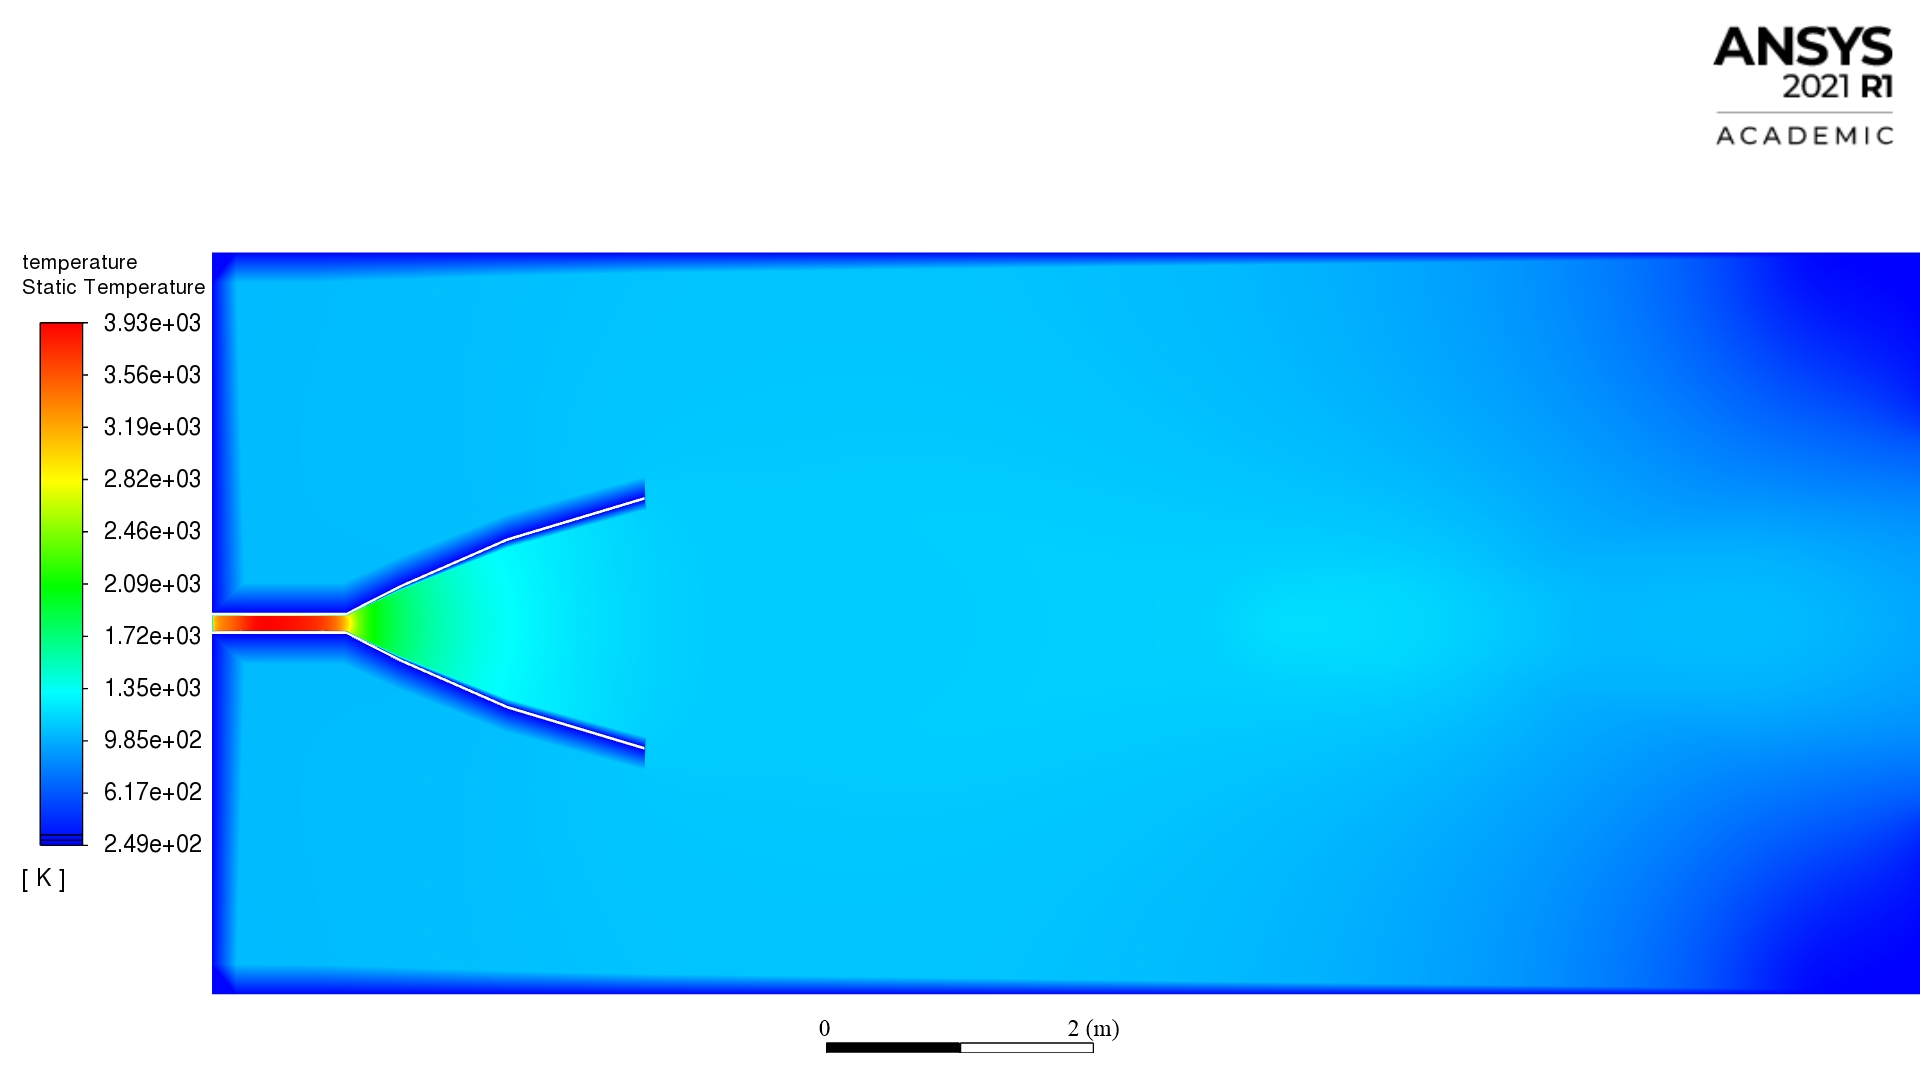
\includegraphics[width=0.7\textheight, angle=0,origin=c]{chapter_3/pure_temperature.jpg}
	\caption{Поле температур (розрахунок без введення присадки, CFD-модель з попереднього дослідження)~\cite{Previous}}
	\label{fig:pure_temperature}
\end{figure}

Верифікація здійснювалась шляхом порівняння тиску та температури у камері, розрахованих у пакеті Fluent (рис.~\ref{fig:pure_temperature}), з отриманими значеннями з розрахунку у пакеті \texttt{Астра.4/рс} (рис.~\ref{fig:Vinci_1perc_pure}) і фактичними значеннями характеристик двигуна. Результати верифікації наведені у табл.~\ref{tab_verification}.

\begin{figure}
	\centering
	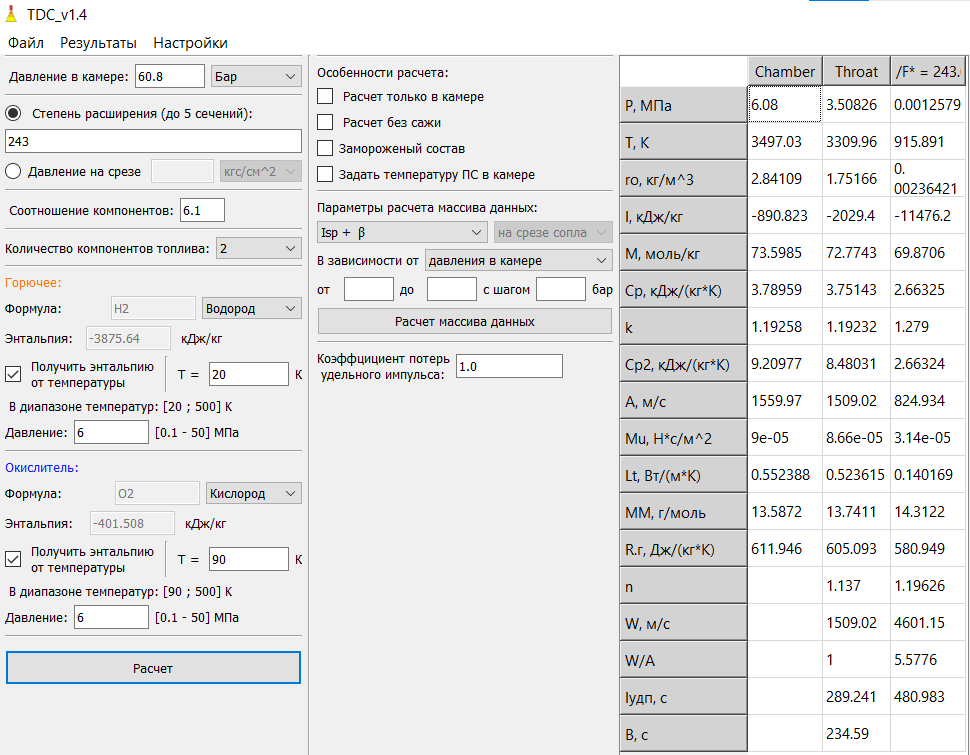
\includegraphics[width=0.7\textheight, angle=0,origin=c]{chapter_2/Vinci_1perc_pure.png}
	\caption{Розрахунок термо- і газодинамічних параметрів камери двигуна ESA Vinci (інтерфейс оболонки програмного комплексу Астра.4/рс )}
	\label{fig:Vinci_1perc_pure}
\end{figure}

\begin{table}[t!]\centering\small
	\caption{Результати верифікації моделі розрахунку у комплексі \texttt{Астра.4/рс} відносно фактичних характеристик РРД ESA Vinci~\cite{VinciData}~\cite{VinciDataDLR} і CFD-моделі \texttt{ANSYS} Fluent}
	\begin{tabular}{|l|c|c|c|c|}
		\hline
		\thead{} & \thead{Література} & \thead{Fluent} & \thead{Астра.4}\\
		\hline
		Тиск у камері, бар & $60.8$ & $80$ & $60.8$\\
		\hline
		Температура у камері, К & $3600$ & $3930$ & $3497$ \\
		\hline
		Відхилення показника тиску, \% & -- & $31.58$ & -- \\
		\hline
		Відхилення температури, \% & -- & $9.17$ & $2.86$ \\		
		\hline
	\end{tabular}
	\label{tab_verification}
\end{table}	


\section{Постановка умов задачі. Розрахунки на основі параметрів існуючих РРД}


Для додаткової верифікації моделі (порівняння з фактичними параметрами існуючих РРД) були розраховані термодинамічні параметри (без додавання присадки) камер декількох ракетних двигунів різних діапазонів потужностей - від кількох тонн (Flight Control SV3, 3 тс) до великих установок для важких ракет-носіїв (РД-120, 85 тс; РД-0120, 200 тс), що можуть бути потенційно застосовані у складі плазморідинного двигуна. За результатами, теоретичні розрахункові параметри РРД, зокрема тяга, питомий імпульс і витратний комплекс (без урахування коефіцієнтів реальних втрат камери, сопла та ін.) відповідають їх характеристикам.

Після верифікації у цьому ж пакеті (застосовуючи ідентичні моделі кінетики взаємодії компонентів) були проведені розрахунки за присутності визначеної масової частки присадки робочого тіла МПД-прискорювача, що складала 2\% від витрати двигуна. За результатами двох розрахунків (камера без присадки і за її присутності) визначався спад параметрів камери РРД. Отримані значення наведені у розділі~\ref{sec:model_results} (табл.~\ref{tab_LPRE}).

%Побудова геометрії задачі здійснена з урахуванням потреби в оптимізації розрахункової області для отримання високої точності розрахунку на доступних обчислювальних потужностях. Оптимальним у такому випадку виявляється 2D~-~вісесиметричний профіль, що і був побудований в окремій програмі та імпортований в пакет \texttt{ANSYS}. Геометричні параметри взяті з технічної документації згаданого РРД $Vinci$ \cite{VinciData}.
%Розрахункова геометрія побудована у $SolidWorks$ $2020$, її вигляд наведено на рис.~\ref{fig:geometry_advanced_screen_new}.



%Розрахункова сітка побудована засобами препроцесора \texttt{ANSYS} $Meshing$; вихідний варіант містить 107562 комірок і 105066 вузлів з основним адаптивним та додатковим локальним розбиттям у ділянках, де потребується згущення (камера згоряння, критичний переріз сопла, область за зрізом стінки і зрізом сопла далі по довжині розрахункової області). Розміри елементів (довжини сторін чотирикутних комірок) в залежності від локального розбиття варіюються від $50$ мкм (критика сопла) до $5$ мм; ділянки обабіч сопла розташовані поза потоком, сітка у них має менше згущення.


\section{Параметри робочого тіла МПД-прискорювача}

 
\begin{figure}[h!]
	\centering
	\subfloat[$5$ мкм]{%
		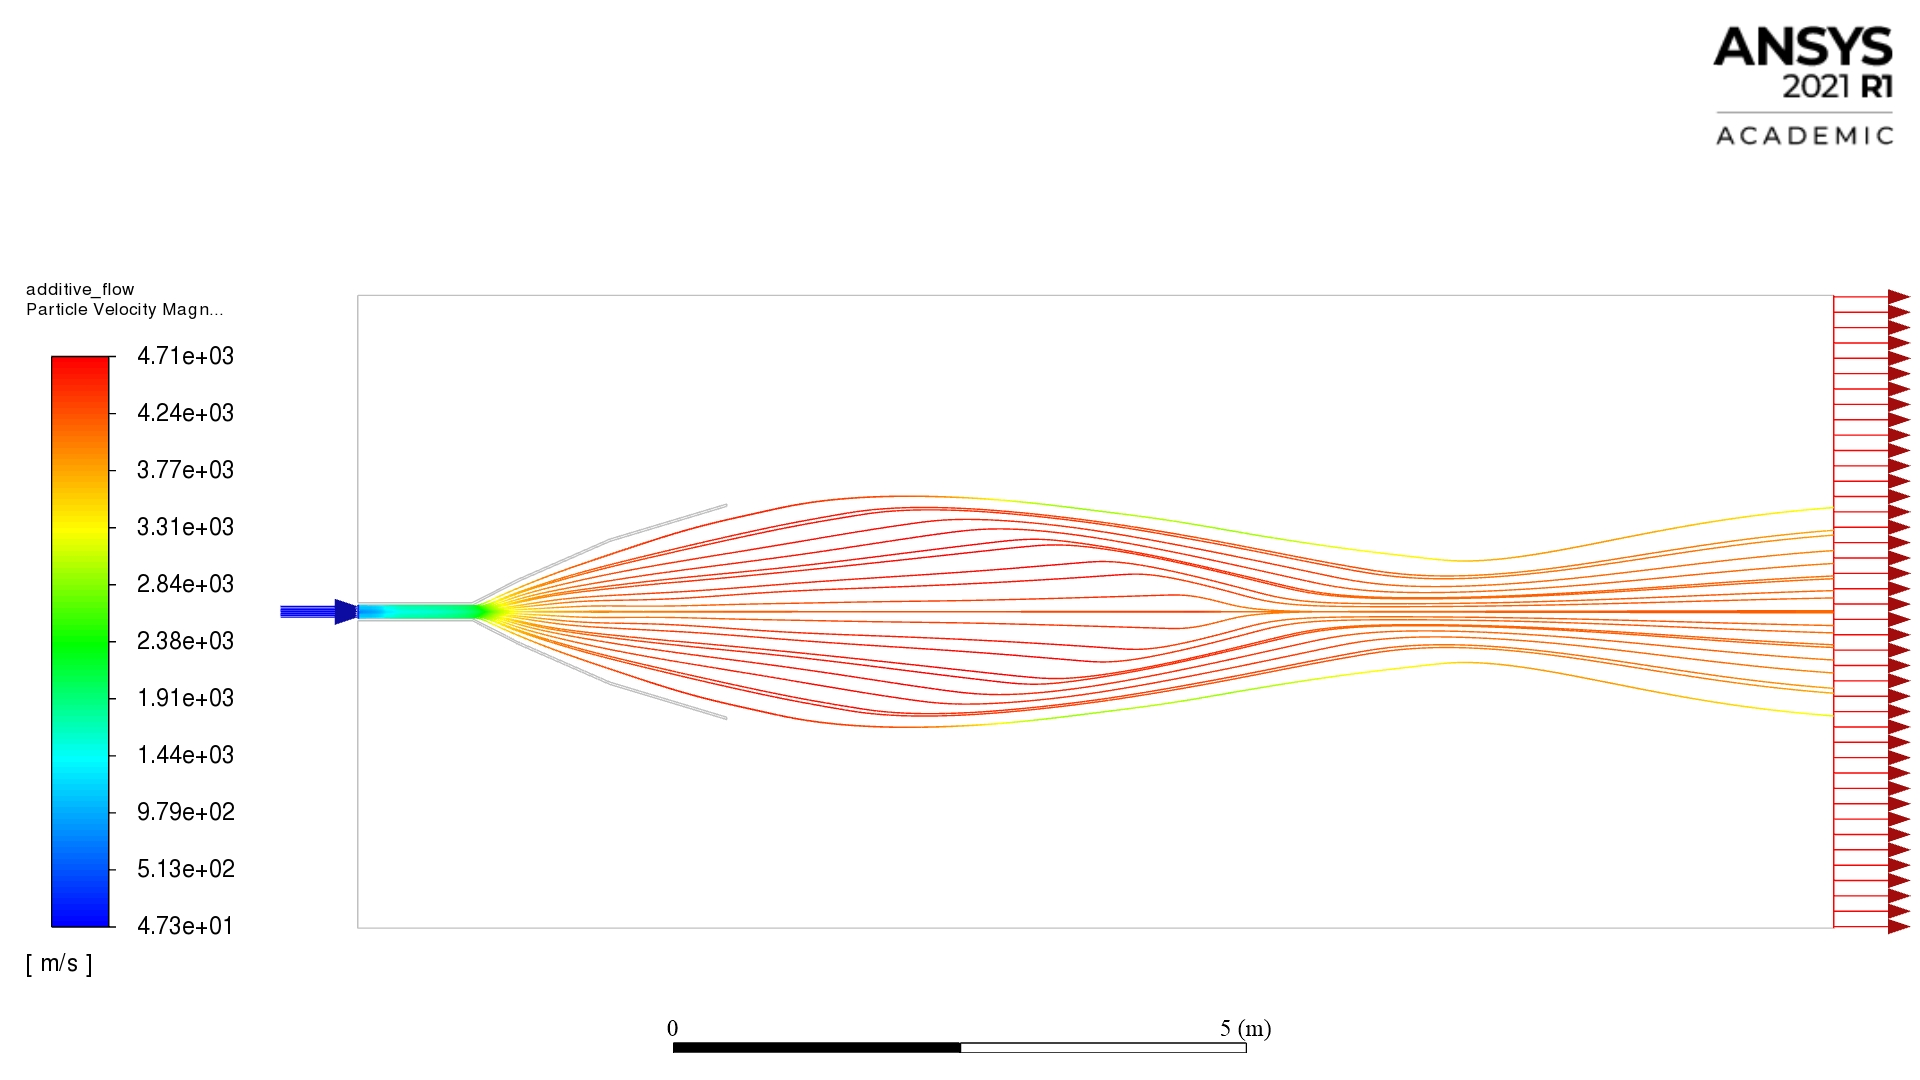
\includegraphics[width=0.4\columnwidth]{chapter_3/additive_5.jpg}
		\label{subfig1}
	}%
	\\ % <- для того, щоб рисунки розташувались в колонку
	\subfloat[$10$ мкм]{
		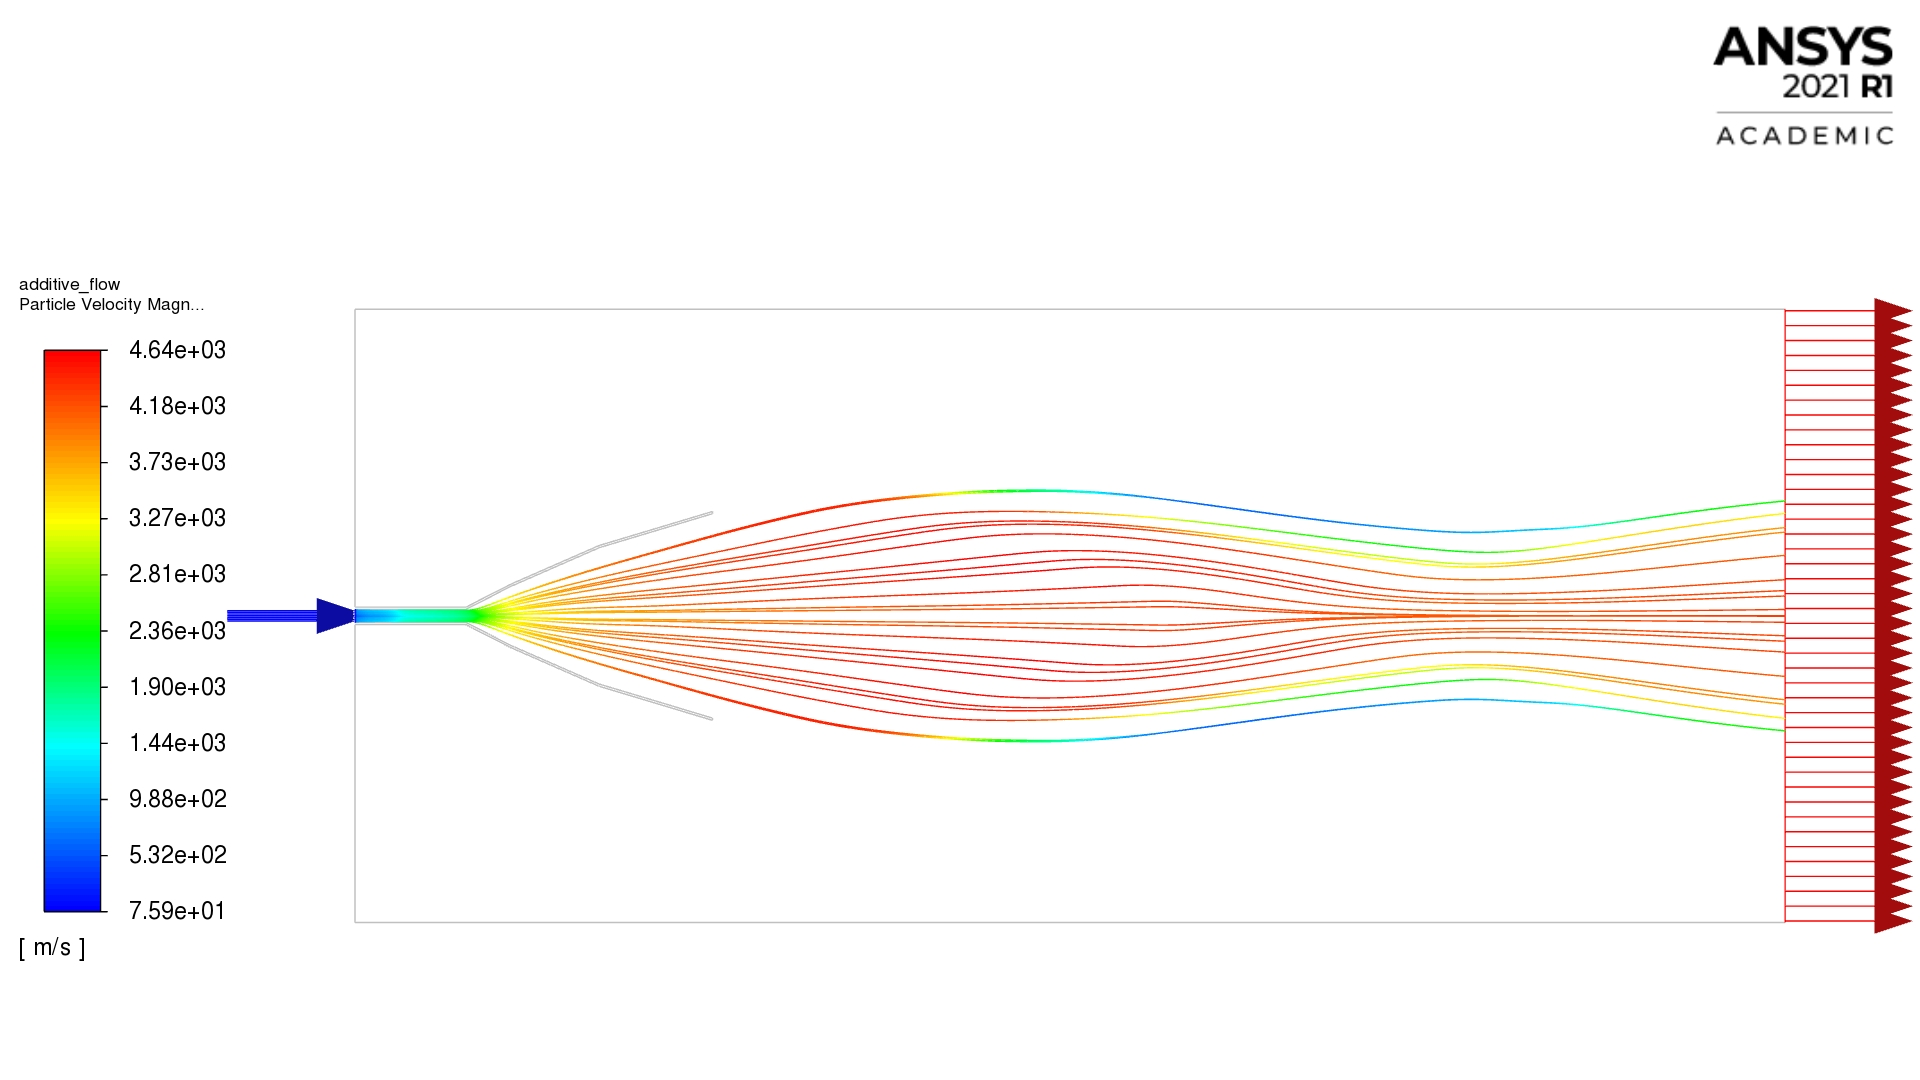
\includegraphics[width=0.4\columnwidth]{chapter_3/additive_10.jpg}
		\label{subfig2}
	}%
	% <- для того, щоб рисунки розташувались в колонку
	\subfloat[$20$ мкм]{
		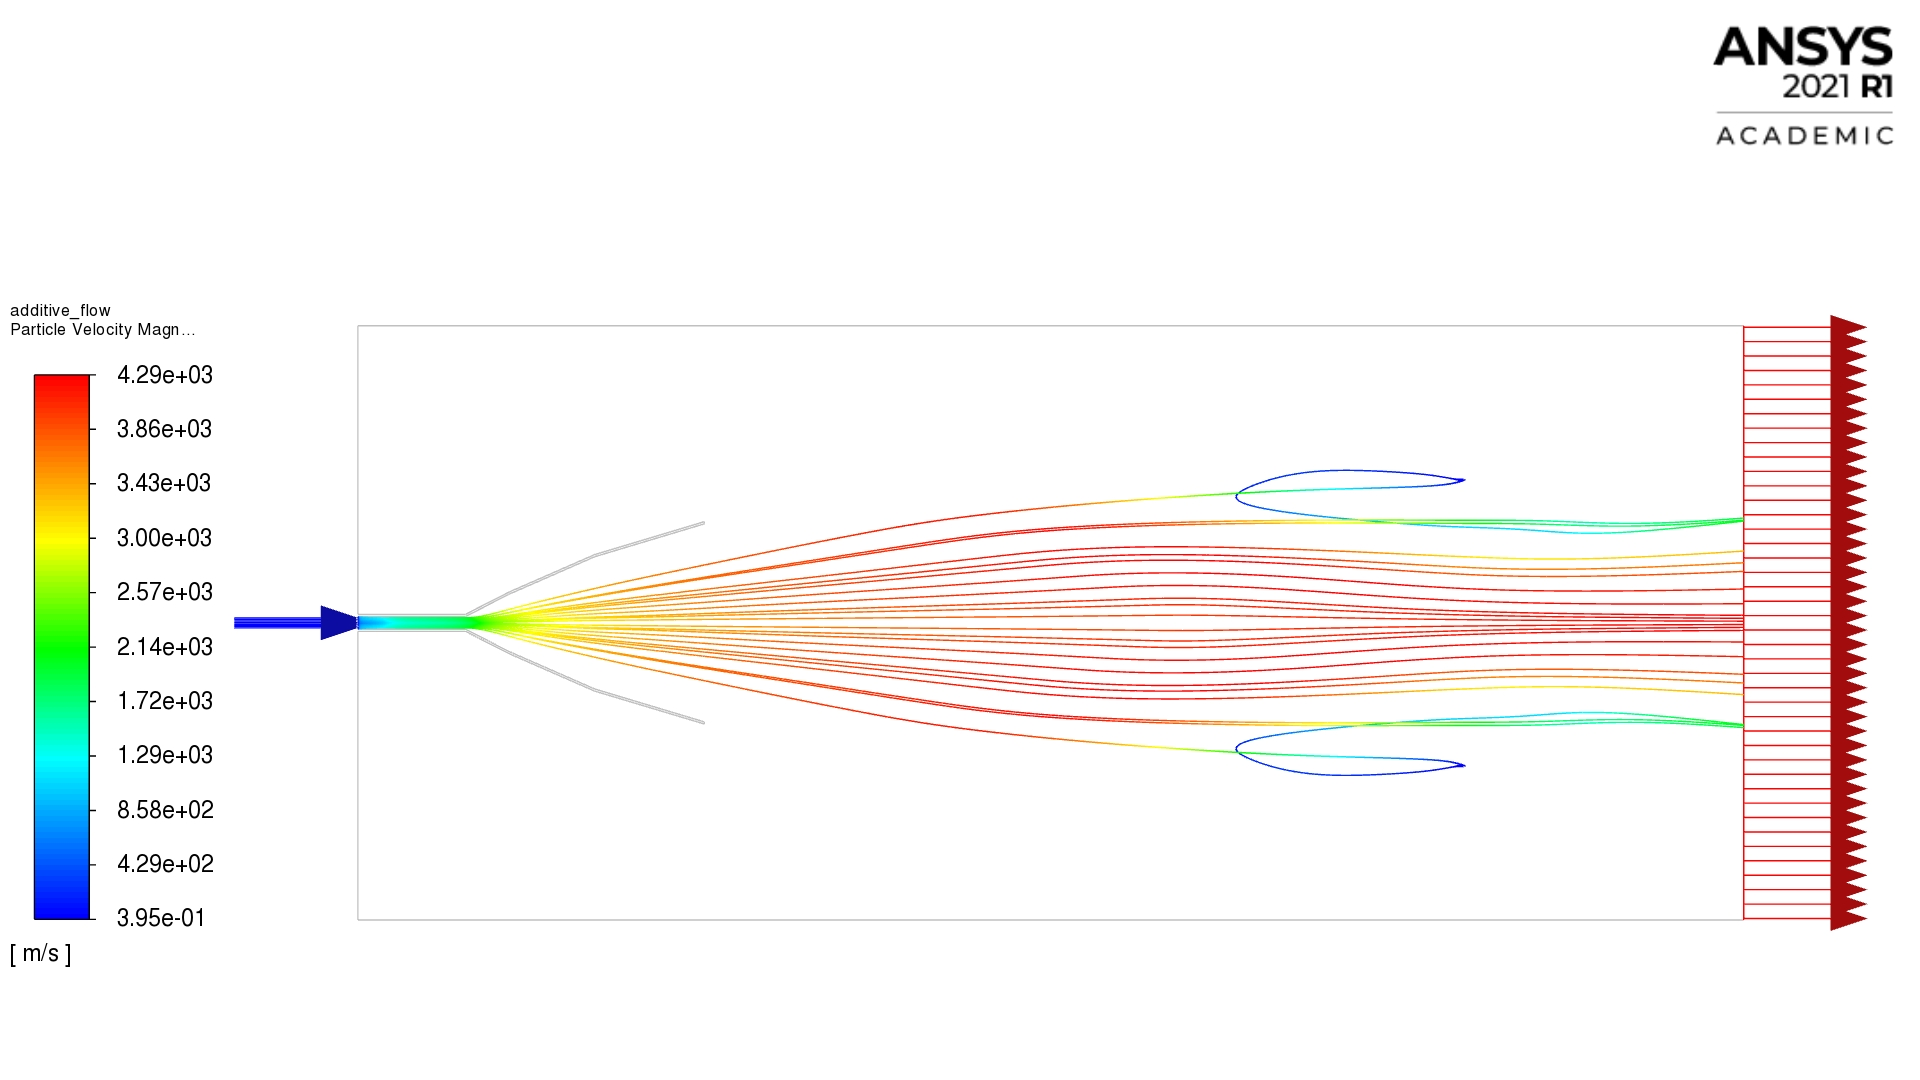
\includegraphics[width=0.4\columnwidth]{chapter_3/additive_20.jpg}
		\label{subfig3}
	}%
	\\ % <- для того, щоб рисунки розташувались в колонку
	\subfloat[$50$ мкм]{
		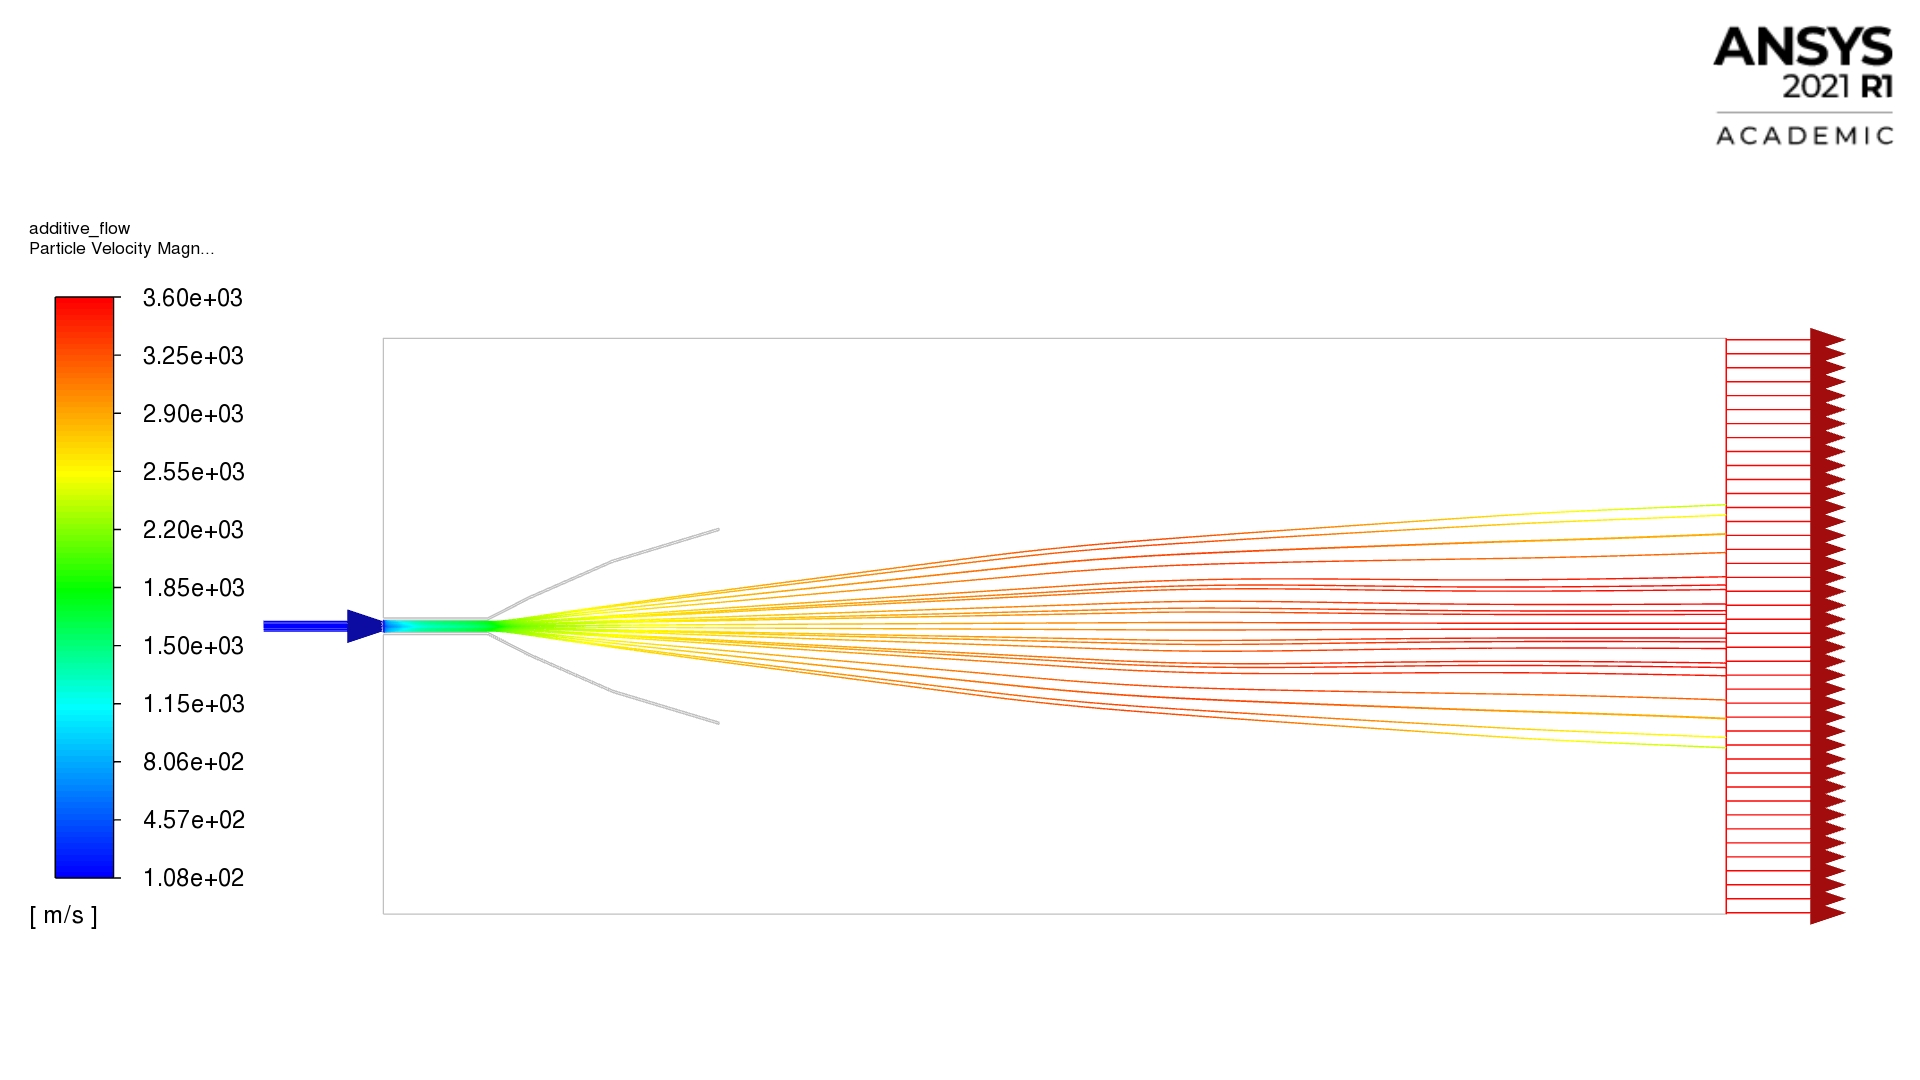
\includegraphics[width=0.4\columnwidth]{chapter_3/additive_50.jpg}
		\label{subfig4}
	}%
	% <- для того, щоб рисунки розташувались в колонку
	\subfloat[$75$ мкм]{
		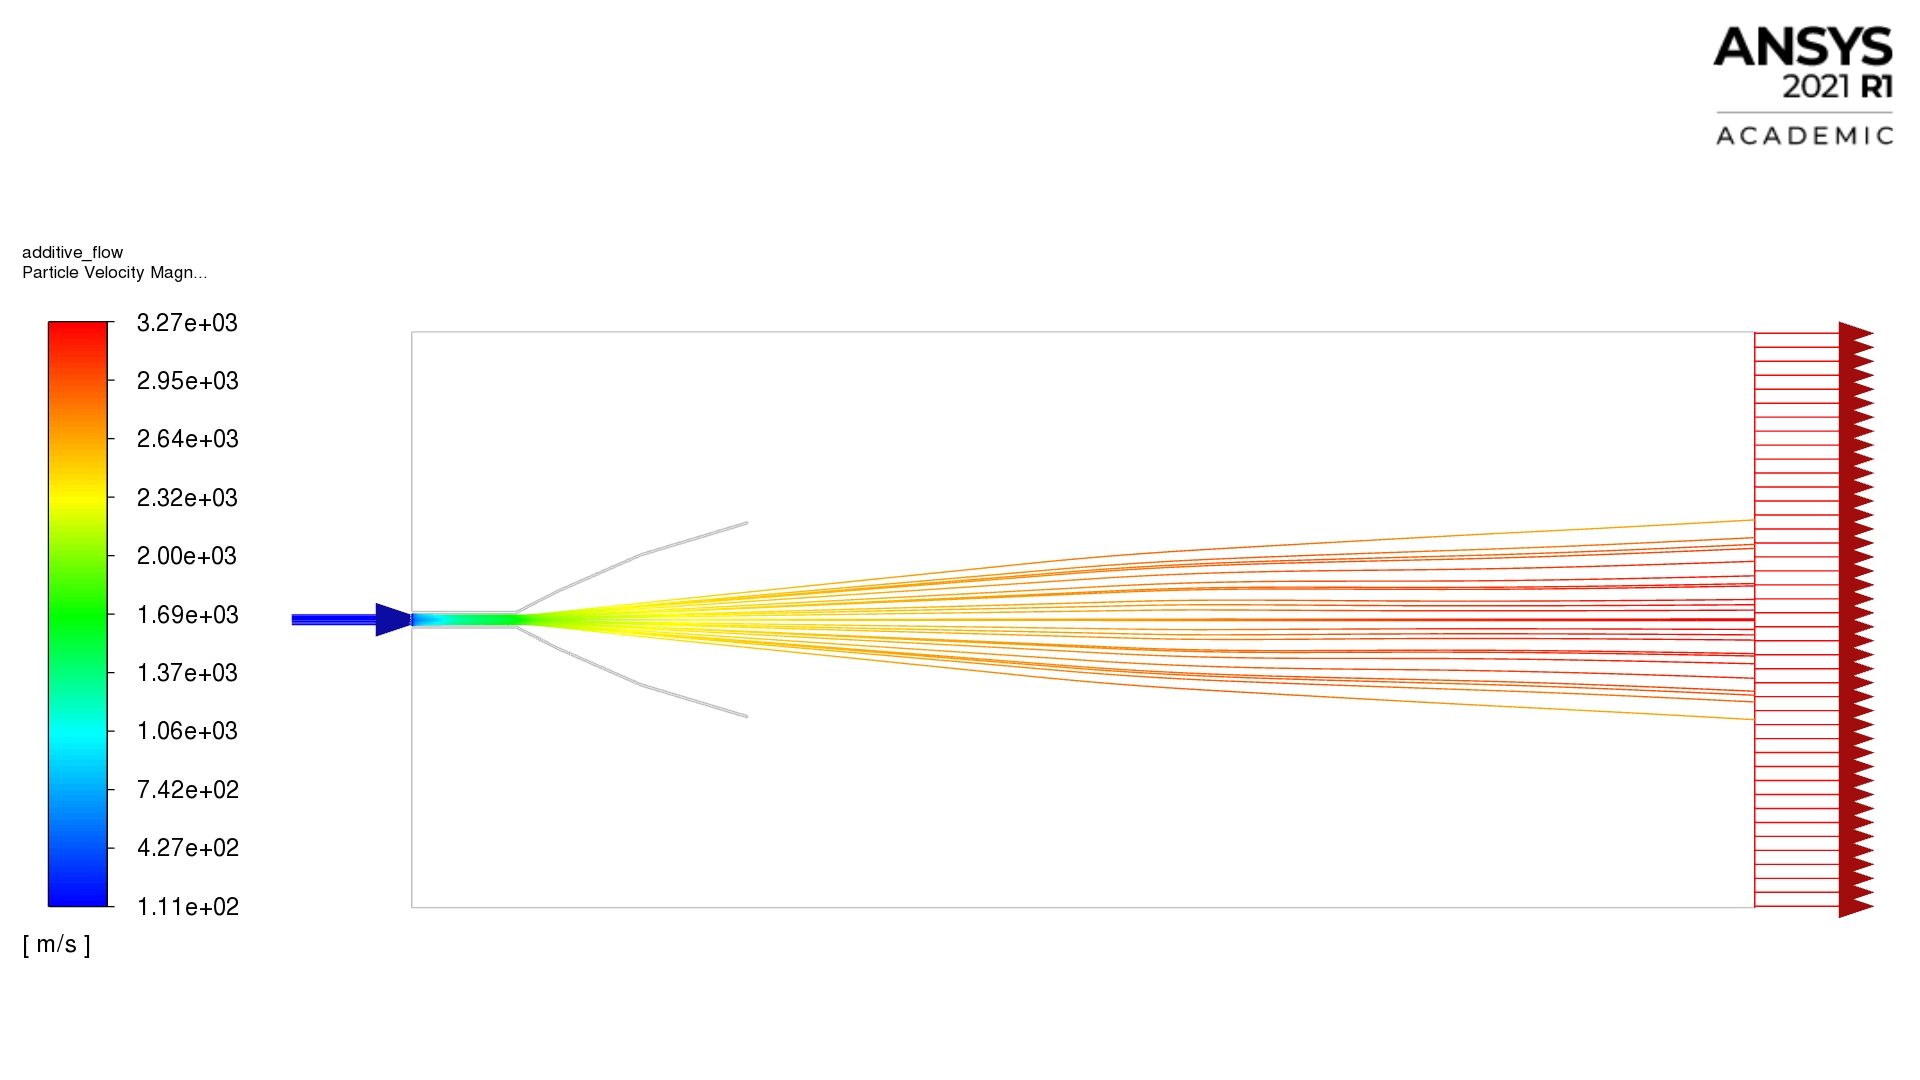
\includegraphics[width=0.4\columnwidth]{chapter_3/additive_75.jpg}
		\label{subfig5}
	}%
	\\
	\caption{Траєкторії частинок присадки калію різних фракцій, введеної в РРД (CFD-модель з попереднього дослідження)~\cite{Previous}}
\end{figure}

У якості робочого тіла МПД-прискорювач використовує дрібнодисперсний порошок калію; подача присадки має здійснюватись з окремої форсунки паралельно з паливними компонентами. Оптимальний розмір частинок був визначений у попередньому дослідженні~\cite{Previous}; спираючись на результати CFD-моделювання, для забезпечення належного прогріву частинок у потоці газу (максимізації температури присадки на виході з камери) і водночас мінімізації можливих процесів ерозії стінки КЗ і сопла розмір частинок присадки доцільно брати рівним 10 мкм (див. рис.~\ref{subfig2}). Для збільшення питомої тяги електроракетної установки частка присадки збільшена до 2\% (0.02 витрати робочого тіла установки; характерне значення, використовуване в МПД-прискорювачах, згідно даних~\cite{Panchenko}, становить від 1 до 10\% для МГД-установок на присадках лужних металів).

\section{Висновки розділу 2}

Для належної точності числового моделювання необхідно застосувати програмний комплекс, що включає у себе моделі поведінки паливних компонентів за умов камери згоряння РРД. Такий комплекс було підібрано, проведена верифікація згідно відомих енергетичних параметрів декількох типів існуючих РРД; було проведене порівняння з CFD -- моделлю для аналогічних розрахунків, виконаною у попередньому дослідженні.

Задача термодинамічного моделювання поведінки паливних сумішей є апробованою, проте має певні особливості (високі значення тисків та температур, наявність активних процесів рекомбінації тощо), що враховуються застосованим програмним комплексом.

Побудована і верифікована відносно параметрів існуючих двигунів модель дозволяє виводити усі основні необхідні параметри енергетичного розрахунку РРД.

Параметри двигунів були опрацьовані вищеозначеним програмним комплексом \texttt{Астра.4/рс}, здійснене моделювання термодинаміки КЗ трьох різних двигунів, проведений їх енергетичний розрахунок.   
\chapter{Результати моделювання. Оцінка характеристик двигуна}\label{sec:model_results}

\section{Результати моделювання термодинамічних процесів у камері РРД}




За допомогою програмного комплексу відкритого доступу \texttt{Астра.4/рс} після верифікації моделі було проведено термодинамічний розрахунок дво- і трикомпонентних реакцій у камері трьох різних РРД, розглянутих у розділі~\ref{sec:model_conditions} за присутності компонентів паливної суміші та визначеної масової частки присадки (рис.~\ref{fig:RD-0120_add},~\ref{fig:11D123_add},~\ref{fig:SV-3_add}). Спад тяги після введення третього компонента розрахований на основі отриманих основних параметрів камери згоряння та сопла: тиску в ядрі потоку, питомого імпульсу, витратного і тягового комплексів та площі критики.

\begin{figure}
	\centering
	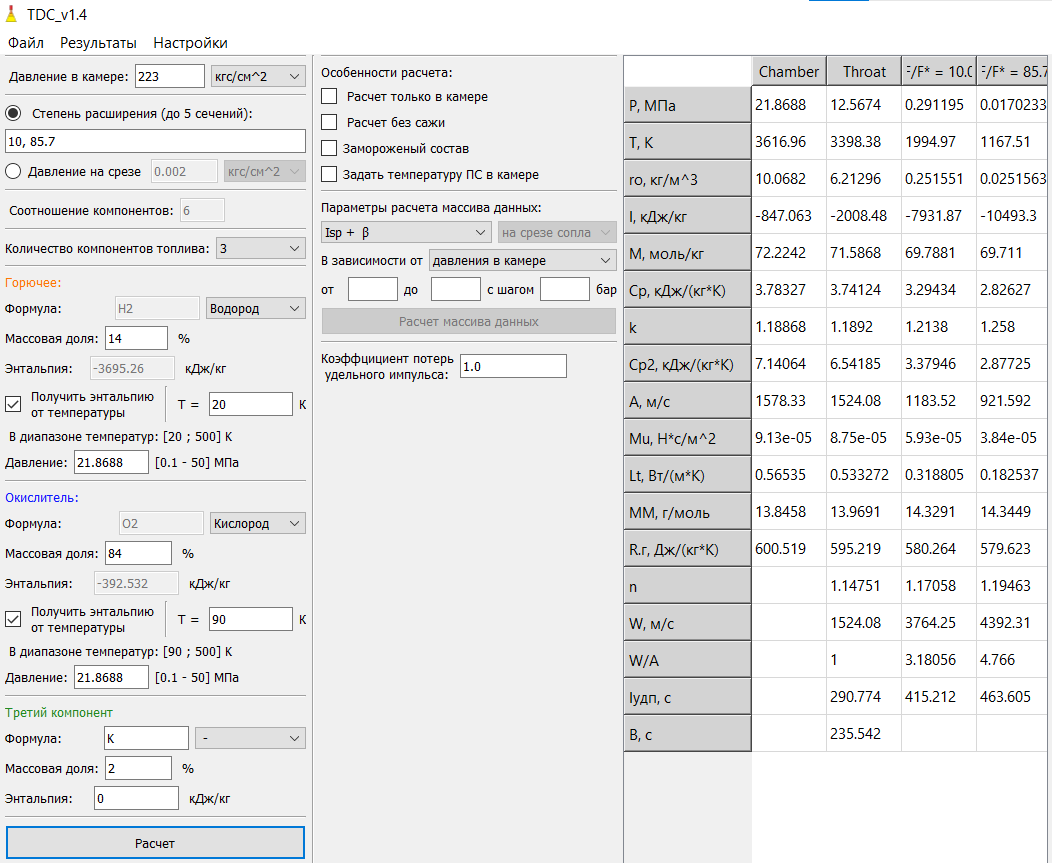
\includegraphics[width=0.5\textheight, angle=0,origin=c]{chapter_3/RD-0120_add.png}
	\caption{Розрахунок термо- і газодинамічних параметрів камери і визначених перерізів сопла двигуна РД-0120 за присутності частинок присадки (інтерфейс оболонки програмного комплексу \texttt{Астра.4/рс})}
	\label{fig:RD-0120_add}
\end{figure}

\begin{figure}
	\centering
	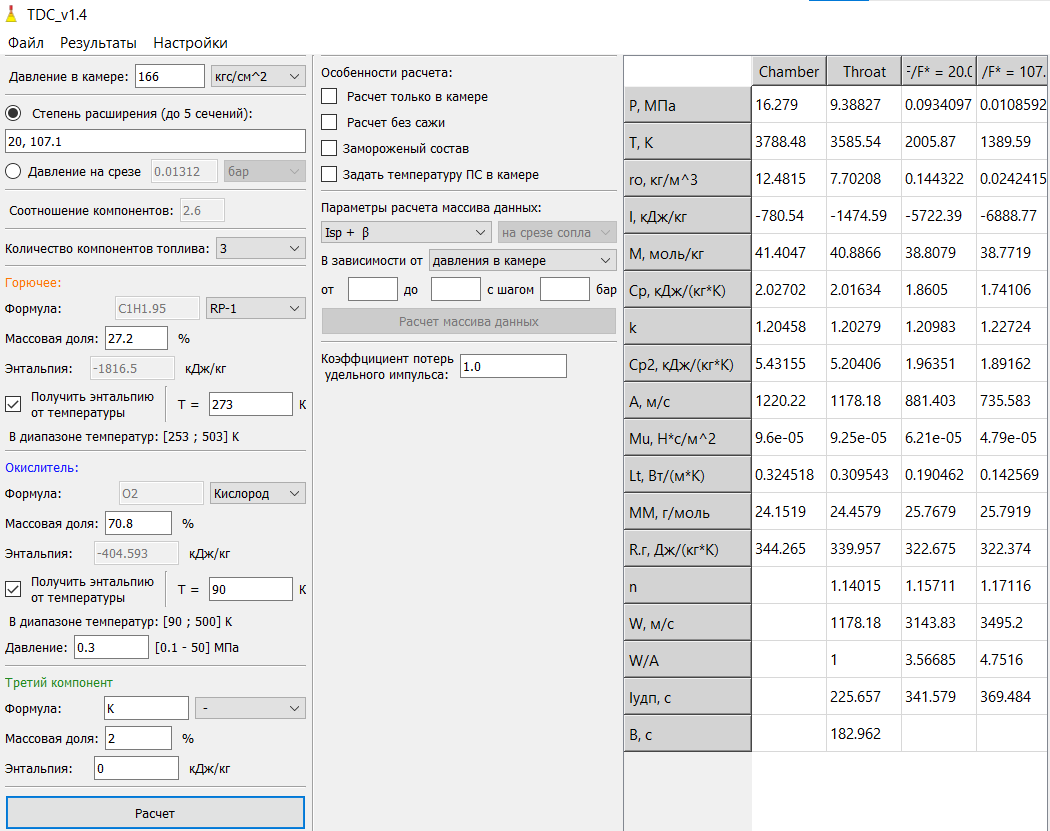
\includegraphics[width=0.5\textheight, angle=0,origin=c]{chapter_3/11D123_add.png}
	\caption{Розрахунок термо- і газодинамічних параметрів камери і визначених перерізів сопла двигуна 11Д123 за присутності частинок присадки (інтерфейс оболонки програмного комплексу \texttt{Астра.4/рс})}
	\label{fig:11D123_add}
\end{figure}

\begin{figure}
	\centering
	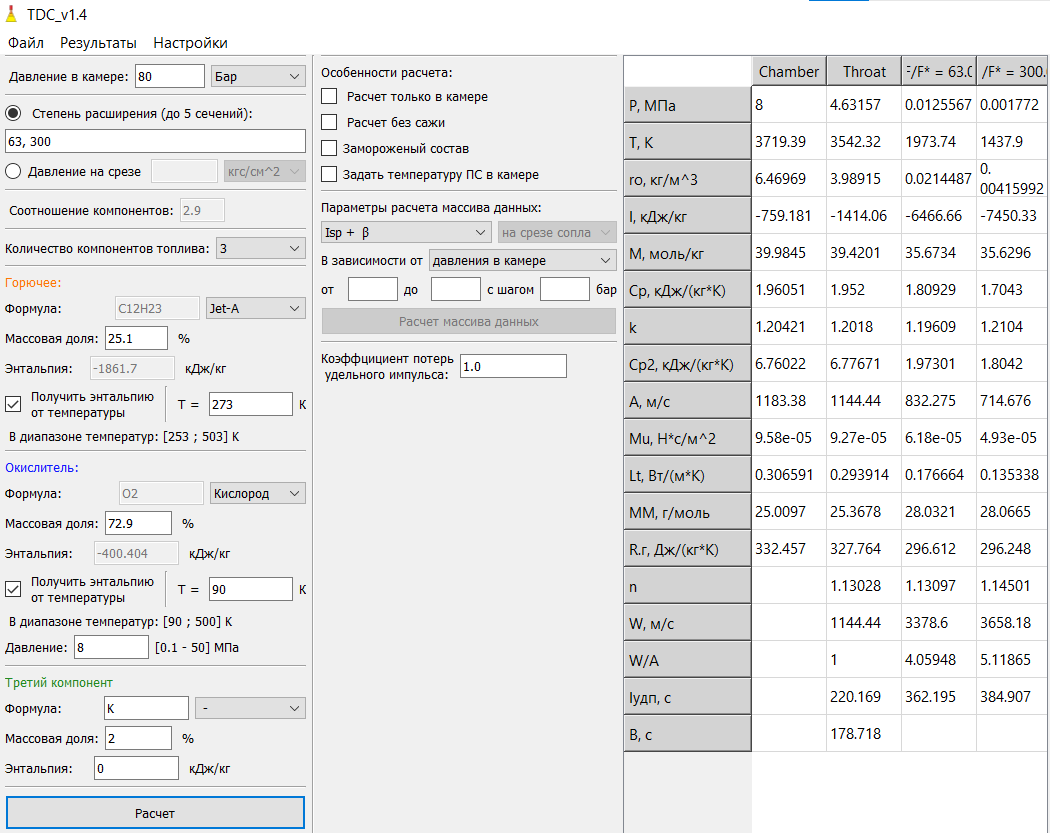
\includegraphics[width=0.5\textheight, angle=0,origin=c]{chapter_3/SV-3_add.png}
	\caption{Розрахунок термо- і газодинамічних параметрів камери і визначених перерізів сопла двигуна SV-3 за присутності частинок присадки (інтерфейс оболонки програмного комплексу \texttt{Астра.4/рс})}
	\label{fig:SV-3_add}
\end{figure}



Результати розрахунку для усіх трьох двигунів наведені у табл.~\ref{tab_LPRE}.

\begin{table}[h!]\centering\small
	\caption{Характеристики РРД за ТД-розрахунком у пакеті \texttt{Астра.4/рс}}
	\begin{tabular}{|l|c|c|c|c|c|c|}
		\hline
		\thead{} & \thead{РД-0120} & \thead{РД-120 (11Д123)} & \thead{Flight Control SV3}\\
		\hline
		Паливо 					& LH2+LOX & РГ-1+LOX & Jet A-1+LOX \\
		\hline
		Маса, кг 				& 3450    & 1125     & 140 \\
		\hline
		Тягооснащеність 		& 57,97   & 75,56    & 21,43 \\
		\hline
		Тяга, тс 				& 200	  & 85       & 3 \\
		\hline
		Питомий імпульс, м/с 	& 4462    & 3432     & 3482,55 \\
		\hline
		Спад тяги з присадкою (\%) & 1,018   & 0,991    & 0,942 \\
		\hline
	\end{tabular}
	\label{tab_LPRE}
\end{table}

%Застосована стандартна ініціалізація розрахунку, задана кількість ітерацій $1000$. Кратність ітерацій DPM - $2$. Верифікаційний розрахунок без введення присадки дійшов збіжності за 429 ітерацій.

%Отримані поля динамічного та повного тиску, температури, швидкості й числа Маха наведені на рис.~\ref{fig:pure_dyn_pressure},~\ref{fig:pure_tot_pressure},~\ref{fig:pure_temperature},~\ref{fig:pure_velocity_magn},~\ref{fig:pure_mach_number}. Помітний перший стрибок ущільнення за зрізом сопла, також наявна вторинна границя потоку. У камері спостерігається вигоряння водню у перших 3-4 см її довжини; далі переважну більшість маси робочого тіла становить вода, проте у перерізі камери тиск і температура досягають значень $8$ МПа і  $3850-3930$ К, близьких до заявлених авторами~\cite{VinciDataDLR} значень для двигуна на режимі, отже задана конфігурація відтворює термо- й газодинамічні параметри РРД.

%Перевірене значення тиску на зрізі сопла свідчить про спад тяги через різницю тисків (англ. pressure thrust) на $29.566$ кН, отже присутнє недорозширення сопла, властиве для двигунів верхніх ступеней та низького тиску навколишнього середовища.

%Проведені розрахунки потоків РРД з введенням частинок калію фракціями 5, 10, 20, 50 і 75 мкм; в результаті отримані траекторії частинок у реактивному струмені РРД, наведені на рис.~\ref{subfig1}~-~\ref{subfig5}. Варто помітити, що зі зменшенням розміру частинок вони рівномірніше розподіляються у перерізі потоку, що може свідчити про наближення до термодинамічної рівноваги між частинками присадки й потоком газу. Наведені траєкторії частинок з профілями швидкості, а також аналогічні траекторії з профілями температури показують, що потоки з присадкою фракцією 5 - 20 мкм мають розподіл значень, близький до розподілу у навколишньому реактивному струмені РРД. Граничні верхні значення у розподілі температур відхиляються у межах 1\%, швидкостей - 0.2, 12.9 і 8.9\% відповідно. У фракції 50 мкм ці відхилення становлять 27\% ($v$) і ті ж 5\% ($T$), для 75 мкм маємо 32.7\% ($v$), 9.2\% ($T$).


\section{Взаємна інтеграція установок і її вплив на результуючі параметри}

\begin{figure}
	\centering
	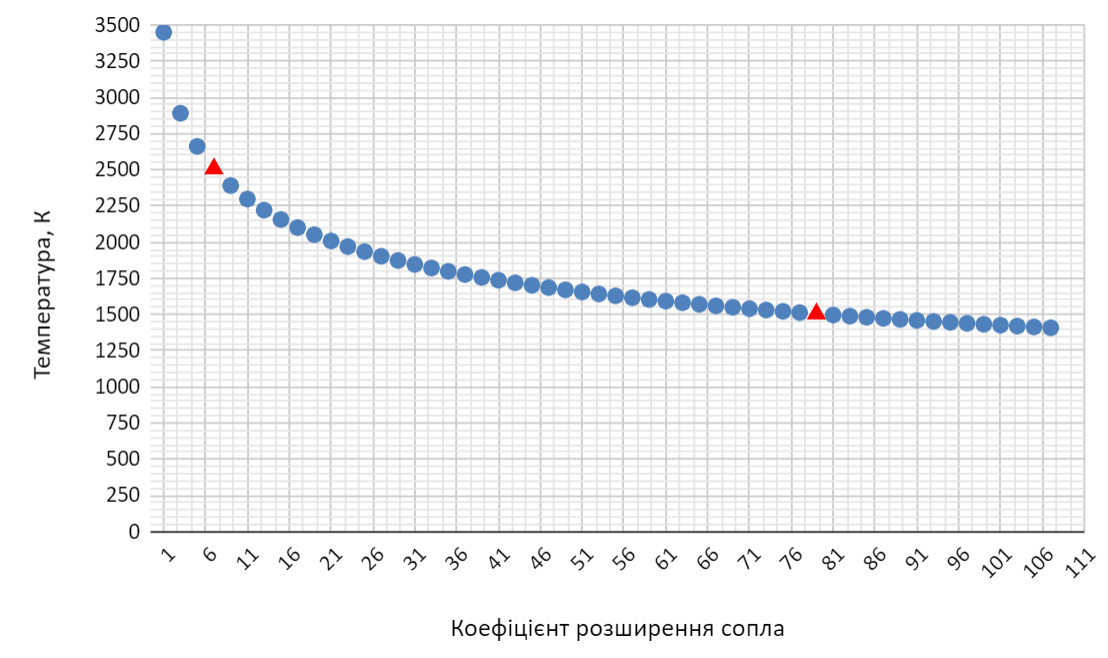
\includegraphics[width=0.7\textheight, angle=0,origin=c]{chapter_3/11D123_T(epsilon).png}
	\caption{Профіль температури у соплі 11Д123; червоним показані перерізи розташування МПД-каналу}
	\label{fig:11D123_T(epsilon)}
\end{figure}

\begin{figure}
	\centering
	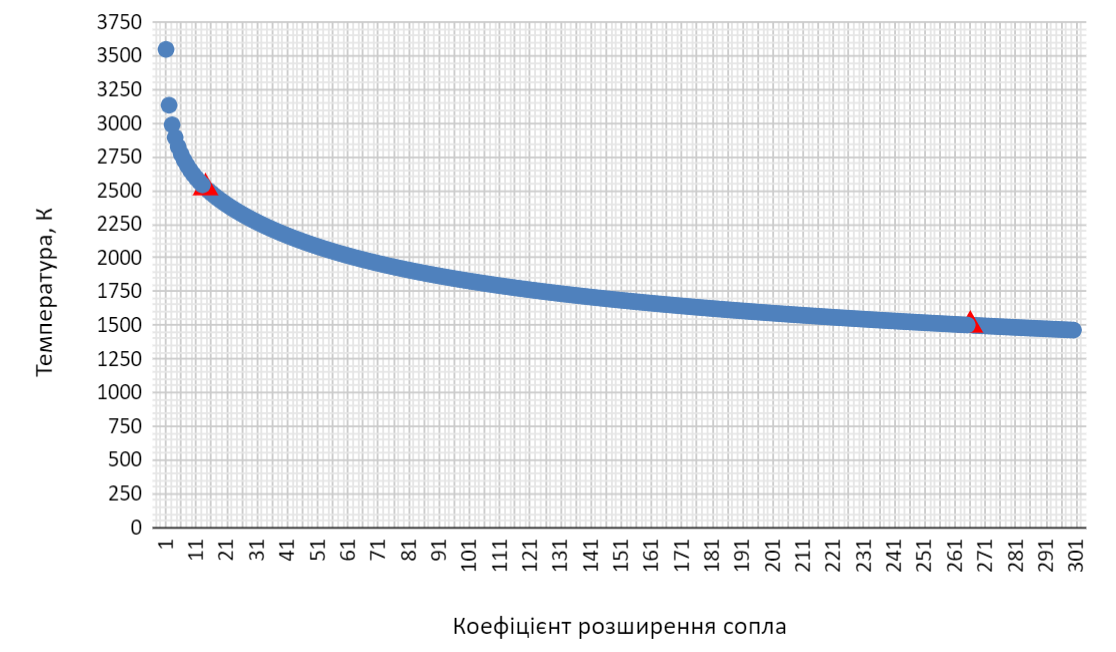
\includegraphics[width=0.7\textheight, angle=0,origin=c]{chapter_3/SV3_T(epsilon).png}
	\caption{Профіль температури у соплі двигуна SV3; червоним показані перерізи розташування МПД-каналу}
	\label{fig:SV3_T(epsilon)}
\end{figure}

\begin{figure}
	\centering
	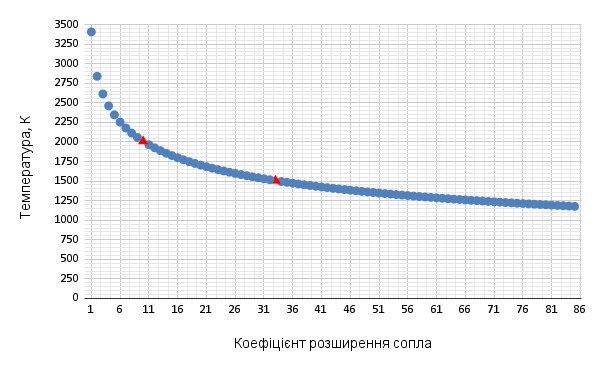
\includegraphics[width=0.7\textheight, angle=0,origin=c]{chapter_3/RD-0120_T(epsilon).png}
	\caption{Профіль температури у соплі РД-0120; червоним показані перерізи розташування МПД-каналу}
	\label{fig:RD-0120_T(epsilon)}
\end{figure}

%Залежність геометрії каналу від температури у соплі як основний чинник зв'язку РРД і МПДП
%Розрахунок в Астрі для визначення взаємного розташування РРД і МГДП (переріз сопла)

Однією з ключових конструктивних проблем рушійної установки, що розглядається у цій роботі, є визначення місця установки МПД-каналу у поздовжньому перерізі РРД. Частинки калію є іонізованими за певних значень температури їх потоку (діапазон $3000 - 1500$~K за даними~\cite{Panchenko}), а отже електромагнітне поле має бути прикладене у перерізі РРД з температурою у цьому діапазоні. Окрім цього з результатів CFD-моделювання у попередньому дослідженні~\cite{Previous} було якісно помічено, що частинки можуть вступати у термодинамічну рівновагу з потоком газу, а отже у критичному перерізі сопла вони набуватимуть швидкості, не більшою за швидкість потоку продуктів згоряння, тому їх електромагнітне прискорення до критики неможливе. Тому у складі плазморідинного двигуна МПД-прискорювач і його канал має бути розташований у закритичному перерізі сопла, на довжину, що відповідає температурі перерізу потоку робочого тіла $1500-3000$~K.

Для визначення меж розташування каналу також був використаний розрахунок з програмного пакету \texttt{Астра.4/рс}: для двигунів за визначеними раніше термодинамічними параметрами (11Д123, SV3 і РД-0120) були отримані профілі температури у ядрі потоку по осі сопла РРД, зображені на рис.~\ref{fig:11D123_T(epsilon}, ~\ref{fig:SV3_T(epsilon)} і ~\ref{fig:RD-0120_T(epsilon)} відповідно. Червоним відмічені перерізи установки каналу у межах, що відповідають ступеню іонізації частинок присадки, близькому до одиниці, за оптимального тиску для роботи МПД-каналу (за даними~\cite{Panchenko}, для лужних металів і температур РРД 10 бар та нижче відповідно).

Після визначення місця розташування МПД-каналу для розглянутих у розділі~\ref{sec:model_conditions} двигунів з урахуванням параметрів МГД-установок, зазначених у~\cite{MHDG}, були розраховані робочі об'єми каналу; ці величини прямо впливають на тягу прискорювача, оскільки ними обмежується переріз, у якому на присадку діє поле електродів та котушок установки.


\section{Оцінка характеристик МПД-прискорювача}

\subsection{Живлення установки\label{sec:power_supply}}

% опис роботи комплексу ТНА+МГДП
Для генерації електромагнітного поля і надання швидкостей робочого тіла у декілька км/с прискорювач потребує підведення потужності порядку мегават. В установці, що розглядається, ця потужність була б доступна на валу системи подачі палива РРД за умови її надлишкової генерації турбіною газогенератора. Проте більшість циклів роботи РРД не дозволяють здійснити відбір потужності (ця проблема розглянута у розділі~\ref{sec:First}).

Для оцінки потужностей, необхідних для отримання високої швидкості витікання МПД-прискорювача, можемо використати термодинамічні параметри двигунів, що розглядались вище (табл.~\ref{tab_LPRE}), а також за допомогою пакету \texttt{Астра.4/рс} розрахувати характеристики газогенератора, необхідного для генерації потужності окремої, паралельної турбіни для живлення МПД-прискорювача. Після генерування потужності на валу турбіни вона може бути перетворена у корисну із застоcуванням синхронного електрогенератора на постійних магнітах -- сучасні установки такого типу дозволяють досягти масової ефективності понад 25 кВт/кг~\cite{PMSG}. Результати оцінки на основі розрахованих ТД-параметрів газогенераторів на відновному газі (потужність турбіни та витрата палива для її роботи) наведені у табл.~\ref{tab_MHD}.

\begin{table}[t!]\centering\small
	\caption{Параметри МПД-установок для РРД різних потужностей (згідно характеристик аналогічних пристроїв~\cite{MHDG})}
	\begin{tblr}{|X[5cm]|Q[3cm]|Q[3cm]|}
		\hline
		& РД-0120 (паралельна турбіна) &  Flight Control SV3 (з водневою турбіною живлення)	\\
		\hline
		Паливо                     & LH2+LOX & Jet A-1+LOX / LH2+LOX \\
		\hline
		Корисна потужність турбіни живлення, МВт                   & 16,817   L &  2,9    \\
		\hline
		Витрата на турбіну живлення (без урахування допалювання), кг/с           & 12,876   & 2,221   \\
		\hline
		Тяга, тс                   & 2,463	 & 1,297  \\
		\hline
		Витрата присадки (частка 2\%), кг/с     & 1,2045    & 0,2079  \\
		\hline
		Швидкість витікання, м/с   & 20054,768  &  61180,736 \\
		\hline
	\end{tblr}
	\label{tab_MHD}
\end{table}



Потужність турбіни живлення залежить від параметрів газу, що поступає на неї з газогенератора (ГГ); чим більшу внутрішню енергію має паливо, тим більша питома потужність установки. Для порівняння були взяті газогенератори двигунів РД-0120 (водневий високого тиску на відновлювальному газі) та 11Д123 (РД-120, паливна пара керосин-кисень, на окиснювальному газі); дані по параметрах газогенераторів взяті з джерел~\cite{Fatuyev, RD-0120}. Оцінка проводилась з огляду на коефіцієнт корисної дії активних турбін РРД розглянутих класів та синхронних генераторів на постійних магнітах. Для водневого газогенератора РД-0120 значення газової сталої продуктів згоряння майже на порядок перевищує цей показник у керосинового ГГ РД-120; потужність на валу водневої турбіни дозволяє отримати прийнятні значення потужності за допустимої витрати палива, керосинова ж турбіна має надто велике споживання. Для 11Д123 з оцінки випливає потреба у витраті на турбіну живлення МПД-установки близько 70\% сумарної витрати самого РРД, що виключає будь-яку доцільність використання МПД-каналу у цьому двигуні.

Витрата палива для генерації корисної потужності у випадку двигуна РД-0120 з урахуванням подальшого допалювання у КЗ становить 12~\% від витрати основної турбіни ТНА РРД. У випадку SV3 воднева турбіна для отримання належної для роботи МПД-каналу густини потужності потребуватиме більше палива, ніж сам РРД (125\% основної витрати двигуна з урахуванням допалювання у КЗ), отже у конструкції цього двигуна застосування МПД-установки також стає недоцільним.

%Отримані результати дають змогу оцінити доцільність використання МПД-прискорювача з огляду на порядок приросту тяги та питомого імпульсу.

%З отриманих значень  температури у камері можемо розрахувати питомий імпульс (теоретичний, без урахування основних втрат, оскільки такі вже були враховані під час моделювання; найбільш значущими є радіаційний теплообмін стінок камери і вплив турбулентності на горіння). Також зі значень швидкості потоку і спаду тиску на зрізі сопла можемо знайти тягу двигуна.


\subsection{Оцінка тяги та швидкості витікання}


%струм на електродах з густини потужності
%потужність прискорювача з геометрії МПД-каналу
%геометрія (довжина каналу) і потужність диктують тягу і швидкість витікання присадки

%Розрахунок потужності МГД-прискорювача граничних параметрів;
%охолодження установки
За умови надання необхідної електричної потужності з генератора на валу турбонасосного агрегата (ТНА) РРД МПД-прискорювач отримує певну частку енергії з циклу рідинного двигуна, перетворюючи її у кінетичну енергію потоку заряджених частинок присадки калію. Тяга, створена таким потоком, незначна внаслідок малої частки присадки у потоці газу, проте вона може мати значно більшу швидкість, що дозволяє отримати більший питомий імпульс установки за умови компенсації втрат на іонізацію калію у потоці робочого тіла РРД.

Маючи розраховану потужність турбіни живлення та корисну потужність, що подається на МПД-канал з генератора (розглянуті у розділі~\ref{sec:power_supply}), можливо оцінити параметри струму на електродах прискорювача і відповідно густину струму в МПД-каналі. Потужність самого прискорювача також диктується геометрією МПД-каналу, оскільки поле створюється у визначеному об'ємі; це визначає силу, яка діє на потік заряджених частинок, що проходять у перерізі каналу і відповідно створюють реактивну тягу, витікаючи з визначеною швидкістю. У рамках оціночного розрахунку рух частинок присадки вважається прямолінійним.

%Розрахунок оптимального співвідношення “тяга-швидкість витікання” для діапазону процентів присадки

\begin{figure}
	\centering
	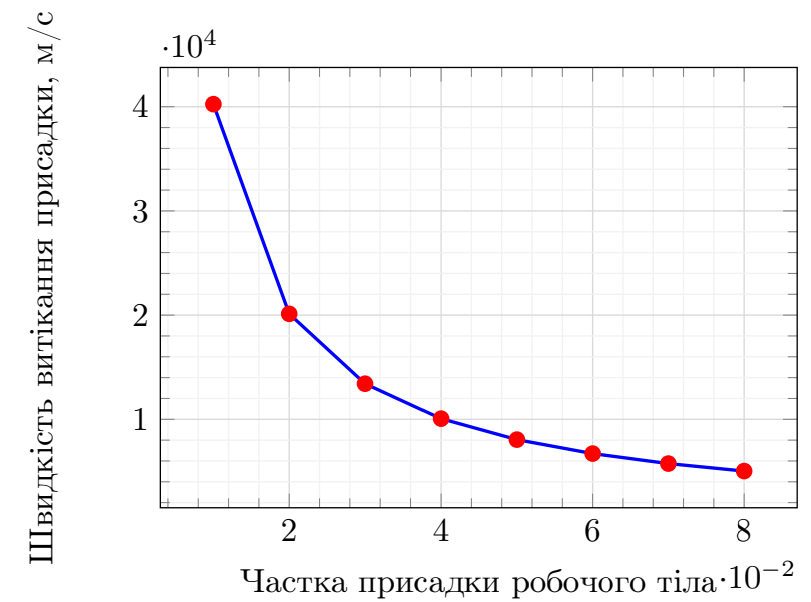
\includegraphics[width=0.5\textheight, angle=0,origin=c]{chapter_3/plot_Isp_WF.png}
	\caption{Графік залежності швидкості витікання робочого тіла МПД-прискорювача від витрати присадки у робочому тілі двигуна (РД-0120, режим низької тяги, РРД дросельований)}
	\label{fig:plot_Isp_WF}
\end{figure}

Тяга МПД-прискорювача була оцінена з виразу для пондеромоторної сили, що діє на електропровідний потік присадки у поздовжньому перерізі на осі МПД-каналу (ідеальний випадок) і утворена взаємодією схрещених електричного та магнітного полів (див. розділ~\ref{sec:First}):

\begin{equation*}
P_{MPD} = j~B \sin{\alpha},
\end{equation*}

де $j$ --- густина струму у перерізі каналу (поздовжньому), $B$ --- індукція котушок, $\alpha$ --- кут між лініями електричного й магнітного полів на осі каналу (конструктивно зумовлено, що на осі МПД-каналу $\alpha = 90\deg$).

Теоретична густина струму на електродах МПД-прискорювача розраховується за формулою (супутніми явищами типу ефекту Холла та ін. нехтуємо):

\begin{equation*}
	j = \frac{I}{F_{el}},
\end{equation*}

де $I$ --- струм на розгінних електродах, $F_{el}$ --- площа поздовжнього перерізу каналу.

Тяга МПД-прискорювача пов'язана з витратою та швидкістю витікання (у випадку електричного ракетного двигуна вона ж є питомим імпульсом у м/с) наступним співвідношенням:

\begin{equation*}
	P_{MPD} = v_{e}~\dot{m}_{MPD},
\end{equation*}

де $v_{e}$ --- швидкість витікання РТ (чисельно дорівнює питомому імпульсу ЕРД), $\dot{m}_{MPD}$ --- масова витрата РТ прискорювача.

Параметри МПД-установки, оцінені згідно геометрії сопла РРД, у якому розташовується МПД-канал, та характеристик створених електричного і магнітного полів, наведені у табл.~\ref{tab_MHD}.

З отриманого перерізу МПД-каналу, використавши електричну потужність прискорювача, можна оцінити густину струму у каналі і відповідно тягу МПД-компонента установки. Для двигуна з-поміж розглянутих вище РРД з допустимою витратою палива для живлення (РД-0120) тяга встановленого у соплі прискорювача становить близько 2,5 тс за значення масової частки присадки 2\%. Тягу можливо підвищити, збільшивши процент присадки, проте це знизить кінетичну енергію потоку РРД і швидкість витікання потоку присадки, оскільки параметри прискорюючого поля диктуються доступною для роботи установки електричною потужністю. Залежність швидкості витікання робочого тіла МПД-прискорювача від частки присадки наведена на рис.~\ref{fig:plot_Isp_WF}.

Результати оцінки (характеристики плазморідинної силової установки на основі РД-0120) наведені у табл.~\ref{tab_PFRE}.

\begin{table}[t!]\centering\small
	\caption{Характеристики гібридної рушійної установки на основі вибраного РРД}
	\begin{tabular}{|l|c|}
		\hline
		& РД-0120 (паралельна турбіна) \\
		\hline
		Частка витрати на турбіну живлення, \% & 2,57 \\
		\hline
		Тяга РРД на другій ступені, тс         &  27,956 \\
		\hline
		Тяга МПД-прискорювача, тс              &  2,463 \\
		\hline
		Швидкість витікання присадки (частка 2\%), м/с   & 20054,768 \\
		\hline
		Питомий імпульс РРД, м/с   							& 4567,977  \\
		\hline
		Приріст питомого імпульсу (РРД + МПД-прискорювач), \%   &   6,67\% \\
		\hline
	\end{tabular}
	\label{tab_PFRE}
\end{table}



В установці пропонується використання надпровідних котушок для зменшення уже наявного (внаслідок близького розташування КЗ) значного теплового навантаження; це дозволить мінімізувати втрату корисної потужності в елементах МПД-прискорювача. Струм на електродах розрахований з потужності, поданої на прискорювач, індукція магнітного поля і напруга підібрані з урахуванням параметрів аналогічних установок~\cite{MHDG}. Ефективність установки можна покращити шляхом додавання контуру регенеративного охолодження котушок; це дозволить збільшити температуру пального на вході у камеру, підвищуючи характеристики РРД на величину порядку 1-2\%.

%Питомий імпульс двигуна розраховується за формулою (подана у~\cite[с. 86]{Walther}):
%\begin{equation*}
%g I_{sp} = v_{e, max} = \sqrt{(n + 2) \frac{R T_{0}} {M_{p}}} ,
%\end{equation*}
%де $g$ --- прискорення вільного падіння, $I_{sp}$ --- питомий імпульс, $v_{e, max}$ --- максимальна ефективна швидкість витікання, $n$ --- показник ступеня свободи молекул газу в суміші продуктів згоряння (у даному випадку для суміші РРД $n = 7,41$), $R$ --- універсальна газова стала, $T_{0}$ --- температура у КЗ, $M_{p}$ --- молярна маса продуктів згоряння (для суміші РТ даного РРД 17,473 г/моль, з урахуванням присадки збільшується до 17,864 г/моль).

%Тяга двигуна розраховується за формулою~\cite[с. 88]{Walther}:
%\begin{equation*}
%F_{t} = \dot{m}_p v_{e} + (p_{e} - p_{\infty}) A_{e},
%\end{equation*}
%де $F_{t}$ ---  тяга, $\dot{m}_p$ --- масова витрата палива, $v_{e}$ --- ефективна швидкість витікання РТ, $p_{e}$ --- тиск на зрізі сопла, $p_{\infty}$ --- тиск навколишнього середовища, $A_{e}$ --- площа соплового зрізу.

%Знак між членами характеризує лише осьову компоненту швидкості (у даному випадку другий доданок з різницею тисків від'ємний через недорозширення сопла).

\section{Перспективи використання РРД з МГД-прискорювачем}

\begin{figure}
	\centering
	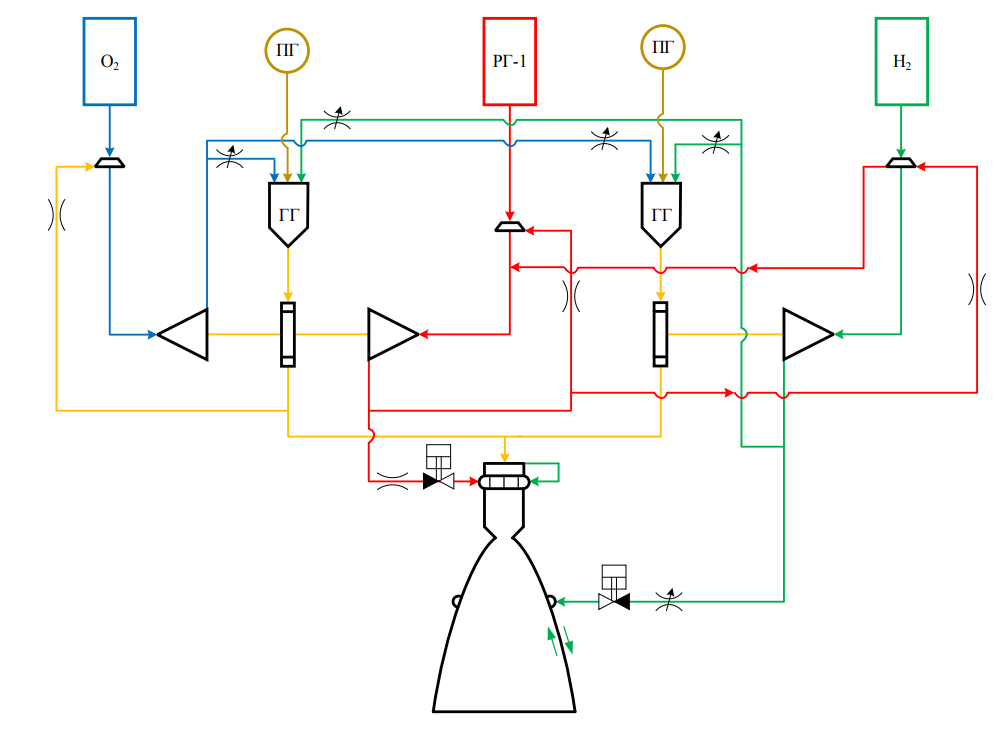
\includegraphics[width=0.6\textheight, angle=0,origin=c]{chapter_3/3comp_engine.png}
	\caption{Принципова схема дворежимного трикомпонентного ракетного двигуна РД-701; на другому режимі використовується воднева турбіна}
	\label{fig:3comp_engine}
\end{figure}

\begin{figure}[h!]
	\centering
	\subfloat[Типовий РРД верхніх ступеней (широкий пунктир)]{%
		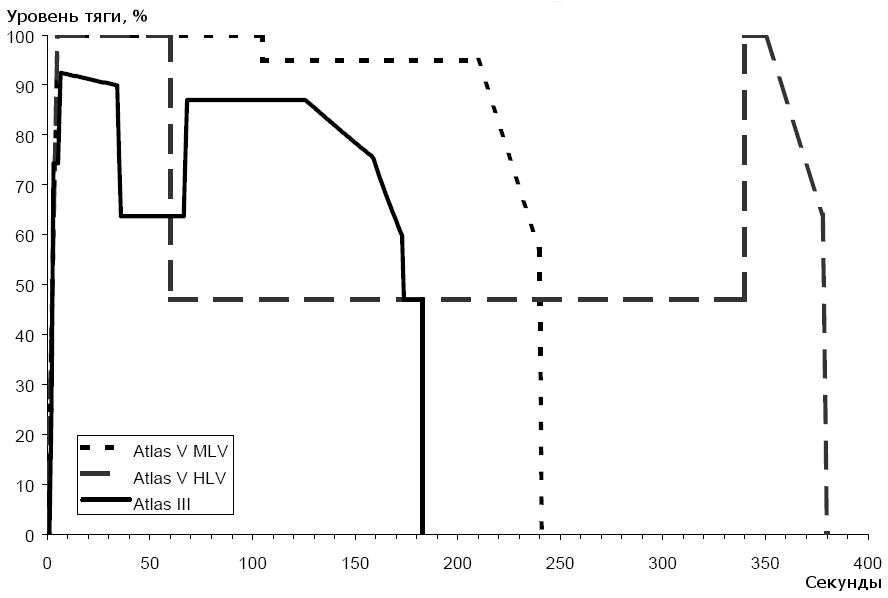
\includegraphics[width=0.6\columnwidth]{chapter_3/RD-180_cyclogram.jpg}
		\label{RD-180_cyclogram}
	}%
	\\ % <- для того, щоб рисунки розташувались в колонку
	\subfloat[Плазморідинний РД]{
		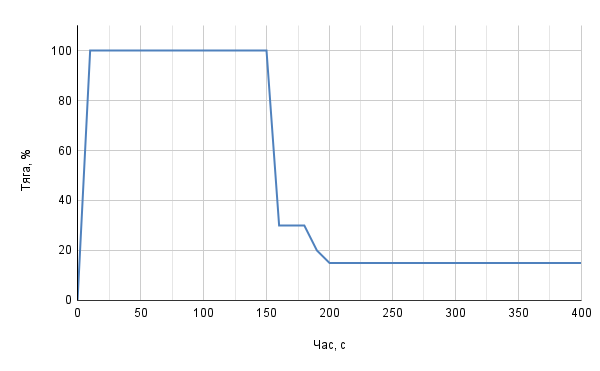
\includegraphics[width=0.6\columnwidth]{chapter_3/thrust_profile_PFRE.png}
		\label{thrust_profile_PFRE}
	}%
	\\
	\caption{Профілі тяги типового РРД верхньої ступені ракети-носія (а) і плазморідинного двигуна у двоступеневій схемі (перша ступінь -- робота РРД, друга ступінь -- глибоко дросельований РРД паралельно з МПД-прискорювачем)}
\end{figure}

%моделювання магнітної системи
%моделювання ерозії критики
%максимізація проценту присадки

Для оцінки параметрів МПД-прискорювача у складі плазморідинного двигуна використовувались зазначені вище три зразки РРД: високоенергетичний великої потужності (РД-0120), висотний керосиновий великої потужності (РД-120) і двигун верхньої ступені з порівняно меншою тягою (Flight Control SV3).

Були розраховані спад тяги і питомого імпульсу РРД внаслідок додавання присадки, корисна потужність на МПД-прискорювач і відповідно отримана тяга та питомий імпульс гібридної установки.

Варто зазначити, що витрати палива для отримання електричної потужності не у всіх трьох розглянутих випадках є оптимальними (у випадку SV3 витрата сягає значень номінальної для РРД на режимі, що виключає можливість ефективного використання ТНА; для 11Д123 МПД-прискорювач недоцільний через неоптимальну геометрію для МПД-каналу у соплі та необхідність додавання масивної водневої паливної системи). Двигун верхньої ступені на парі LH2 + LOX може бути більш придатним для використання у складі розглянутої електрохімічної рушійної установки.

Для компенсації втрат ентальпії потоку продуктів згоряння РРД в установці наявна можливість догріву пального окремим контуром регенеративного охолодження для компенсації спаду імпульсу (у випадку SV3 нагрів на $200$~К повністю компенсує втрату тяги камери).

Існує альтернативний цикл роботи РРД --- трикомпонентна схема, за якої використовуються два ТНА для трьох різних компонентів палива (це дозволяє підвищити масову ефективність і питомий імпульс на різних ділянках польоту, використовуючи два різних види пального з одним окиснювачем) (рис.~\ref{fig:3comp_engine}). Другий ТНА цього двигуна можна використати під час його простою для отримання потужності для МПД-прискорювача, таким чином РРД стає однорежимним (рис.~\ref{RD-180_cyclogram}), або ж має два режими (рис.~\ref{thrust_profile_PFRE}):

\begin{itemize}
	\item великої потужності (працюють обидва ТНА, МПД-прискорювач вимкнено);
	\item високоефективний режим малої тяги (працює один ТНА на більш високоенергетичному компоненті + МПД-прискорювач).
\end{itemize}

Існує протестований зразок дворежимного трикомпонентного двигуна на компонентах РГ-1 + LH2 + LOX --- РД-0750~\cite{RD-0120}. За попередньою оцінкою, використовуючи другий водневий газогенератор такого РРД, можна отримати потужність для МПД-прискорювача порядку 15\% від потужності ТНА спряженого РРД. Для випадку газогенератора РД-0750 витрата, необхідна для отримання потужності, що подаватиметься на МПД-прискорювач, становить близько 13\% витрати двигуна на номінальному режимі.

Отримані результати дають змогу оцінити доцільність використання МПД-прискорювача з огляду на порядок приросту тяги та питомого імпульсу РРД у розглянутій гібридній рушійній установці.

Наведена оцінка потребує подальшого уточнення за допомогою CFD-моделювання МПД-каналу у поєднанні з газодинамічним трактом РРД і взаємодії прискорених іонізованих частинок присадки з надзвуковим потоком продуктів згоряння РРД за наявності схрещених електричного та магнітного полів. Також потребується врахування складної конструкції магнітної системи котушок складної форми (вигнутої по формі сопла РРД). Важливим є питання ерозії стінок камери і сопла за присутності калію для оцінки ресурсу роботи рушійної установки визначених параметрів. Уточнення вищеозначених аспектів моделі дозволить оптимізувати співвідношення робочих тіл РРД і МПД-прискорювача, збалансувавши тягу та питомий імпульс складових розглянутого концепту рушійної установки літального апарата.


\section{Висновки розділу 3}

%Проведене дослідження зміни тяги та питомого імпульсу РРД при введенні у камеру присадки калію шляхом моделювання двофазного потоку з дискретною фазою та виведення основних його характеристик для отримання відповідних параметрів двигуна.

Наведені результати енергетичного розрахунку та термодинамічних параметрів трьох різних РРД, без введення присадки та за її наявності. Розрахований спад тяги двигунів, пов'язаний з введенням робочого тіла МПД-установки у паливну суміш.

На основі результатів ТД-розрахунку були виведені профілі температур по осі сопла, що дозволило розрахувати доступний об'єм МПД-каналу для прискорювача.

Була розрахована потужність турбіни живлення МПД-прискорювача на основі характеристик водневого газогенератора двигуна РД-0120, була оцінена доступна електрична потужність для плазморідинного двигуна.

Було визначено тягу та питомий імпульс МПД-прискорювача для двигуна РД-0120; окреслено недоцільність компонування МПД-компонентом двох інших РРД внаслідок надмірної витрати палива для живлення.

Результати моделювання та подальшої кількісної оцінки свідчать про те, що приріст ефективності плазморідинного двигуна залежить у першу чергу від доступної для МПД-прискорювача потужності, для масових часток присадки порядку декількох процентів витрати РРД спад характеристик рідинного двигуна є незначним, проте для істотного підвищення параметрів МПД-компонента необхідна значно більша потужність, ніж може дати паралельно встановлена воднева газова турбіна.

При розв'язанні проблеми компактного енергоносія для ЕРД плазморідинний двигун може бути ефективним дворежимним РД верхньої ступені ракети-носія внаслідок високої швидкості витікання робочого тіла установки.
\chapter*{Висновки}

\addcontentsline{toc}{chapter}{ВИСНОВКИ}% Додаємо його в зміст

У даному дослідженні проведена оцінка приросту ефективності гібридної електрохімічної ракетної рушійної установки у порівнянні з сучасними рідинними двигунами, що використовуються у ракетах-носіях у даний момент.

Проаналізувавши існуючі конструкції турбоагрегатів РРД, зроблено висновок, що схеми відкритого, закритого (з допалюванням) циклів і циклу з фазовим переходом є малопридатними для використання у якості компонента плазморідинного двигуна.

Було проведено термодинамічний розрахунок дво- і трикомпонентних реакцій у камері плазморідинного двигуна за допомогою програмного комплексу відкритого доступу \texttt{Астра.4/рс}.

Було визначено, що проблема енергообміну між паливною системою РРД і МПД-прискорювачем у випадку живлення останнього від згенерованої потужності на валу турбіни є комплексною і ключовою у даній установці. Використання компактного джерела енергії мегаватної потужності дозволить підвищити тягу МПД-прискорювача, не знижуючи його питомий імпульс.

Схема з паралельною водневою турбіною для живлення МПД-установки і трикомпонентна схема, з конструктивних міркувань, були визначені як оптимальні для компонування з МПД-прискорювачем, оскільки містять додатковий турбоагрегат, що не зазнаватиме критичних навантажень і зумовлює дворежимність установки --- цей фактор може суттєво розширити сферу використання двигуна.

Описаний концепт рушійної установки літального апарата за належної оптимізації та застосування компактного джерела електроенергії для живлення МПД-прискорювача може бути використаний в якості двигуна верхньої ступені або розгінного блоку ракети-носія, в умовах, де необхідний передусім значний питомий імпульс. 


%========================================================================================================

%========================================================================================================

%\clearpage
%========================================================================================================
%
%									       Вставка бібліографії
%
%========================================================================================================
\phantomsection
\pagestyle{main}
\printbibliography[heading=bibintoc]

\appendix
\section{Параметри реакцій горіння палива РРД (\ce{LH2 - LOX})}


    




{\small
\begin{longtable}{|l|c|c|c|c|c|c|l|}
		\caption{Схема протікання реакції горіння водню в умовах, наближених до умов камери згоряння РРД~\cite[с. 384]{Shimizu}\label{chem_kin_h2}}\\\hline
		\thead{№} & \thead{Реакція} & \thead{A} & \thead{$n$} & \thead{$E_a$} & \thead{$F_c$} & \thead{Параметри\\ ефективності}  \\\hline
	    \endfirsthead
	    \caption*{Продовження~табл.~\ref{chem_kin_h2}}\\\hline
		\thead{№} & \thead{Реакція} & \thead{A} & \thead{$n$} & \thead{$E_a$} & \thead{$F_c$} & \thead{Параметри\\ ефективності}  \\\hline
        \endhead
		1 & \ce{OH + H2 = H2O + H} & $2.160\cdot 10^8$ & {$1.51$} & {$3440$} & -- & --  \\
		\hline
		2 & \ce{H + O2 = OH + O} & $1.910\cdot 10^{14}$ & {$0$} & {$16440$} & -- & --  \\
		\hline
		3 & \ce{O + H2 = OH + H} & $5.080\cdot 10^4$ & {$2.67$} & {$6292$} & -- & --  \\
		\hline
		4 & \ce{OH + HO2 = H2O + O2} & $2.890\cdot 10^{13}$ & {$0$} & {$-500$} & -- & --  \\
		\hline
		5 & \ce{H + HO2 = H2 + O2} & $3.660\cdot 10^6$ & {$2.09$} & {$-1450$} & -- & --  \\
		\hline
		6 & \ce{H + HO2 = OH + OH} & $7.080\cdot 10^{13}$ & {$0$} & {$300$} & -- & --  \\
		\hline
		7 & \ce{H + HO2 = H2O + O} & $1.340\cdot 10^{13}$ & {$0$} & {$1340$} & -- & --  \\
		\hline
		8 & \ce{O + HO2 = O2 + OH} & $3.250\cdot 10^{13}$ & {$0$} & {$0$} & -- & --  \\
		\hline
		9a & \ce{HO2 + HO2 = H2O2 + O2} & $4.200\cdot 10^{14}$ & {$0$} & {$12000$} & -- & --  \\
		\hline
		9b & \ce{HO2 + HO2 = H2O2 + O2} & $1.320\cdot 10^{11}$ & {$0$} & {$-1192$} & {$0.5$} & \makecell[l]{Однакові\\ для усіх\\ компонентів}  \\
		\hline
		9c & \makecell[c]{\ce{HO2 + HO2 + M =}\\ \ce{= H2O2 + O2 + M} }& $6.890\cdot 10^{14}$ & {$0$} & {$-1947$} & {$0.5$} & \makecell[l]{Однакові\\ для усіх\\ компонентів}  \\
		\hline
		10 & \ce{OH + OH = O + H2O2} & $4.330\cdot 10^3$ & {$2.7$} & {$-2485$} & -- & --  \\
		\hline
		11 & \ce{H2O2 + H = H2O + OH} & $8.190\cdot 10^8$ & {$1.55$} & {$3455$} & -- & --  \\
		\hline
		12a & \ce{H2O2 + H = HO2 + H2} & $8.067\cdot 10^{19}$ & {$-1.574$} & {$16838$} & -- & --  \\
		\hline
		12b & \ce{H2O2 + H = HO2 + H2} & $1.042\cdot 10^{13}$ & {$0$} & {$6569$} & -- & --  \\
		\hline
		13a & \ce{H2O2 + OH = H2O + HO2} & $1.700\cdot 10^{18}$ & {$0$} & {$29407$} & -- & --  \\
		\hline
		13b & \ce{H2O2 + OH = H2O + HO2} & $2.000\cdot 10^{12}$ & {$0$} & {$427$} & -- & --  \\
		\hline
		14 & \ce{H2O2 + O = HO2 + OH} & $6.620\cdot 10^{11}$ & {$0$} & {$3974$} & -- & --  \\
		\hline
		15a & \ce{H + O2 = HO2} & $1.933\cdot 10^{12}$ & {$0.56$} & {$0$} & {$0.62$} & --  \\
		\hline
		15b & \ce{H + O2 + M = HO2 + M} & $4.570\cdot 10^{18}$ & {$-1.12$} & {$0$} & {$0.62$} & --  \\
		\hline
		15c & \ce{H + O2 = HO2} & $1.933\cdot 10^{12}$ & {$0.56$} & {$0$} & {$0.5$} & --  \\
		\hline
		15d & \ce{H + O2 + H2 = HO2 + H2} & $3.520\cdot 10^{18}$ & {$-0.896$} & {$0$} & {$0.5$} & --  \\
		\hline
		15e & \ce{H + O2 = HO2} & $1.933\cdot 10^{12}$ & {$0.56$} & {$0$} & {$0.67$} & --  \\
		\hline
		15f & \ce{H + O2 + N2 = HO2 + N2} & $1.750\cdot 10^{19}$ & {$-1.232$} & {$0$} & {$0.67$} & --  \\
		\hline
		15g & \ce{H + O2 = HO2} & $1.933\cdot 10^{12}$ & {$0.56$} & {$0$} & {$0.5$} & --  \\
		\hline
		15h & \ce{H + O2 + O2 = HO2 + O2} & $1.410\cdot 10^{18}$ & {$-0.849$} & {$0$} & {$0.5$} & --  \\
		\hline
		15i & \ce{H + O2 = HO2} & $1.933\cdot 10^{12}$ & {$0.56$} & {$0$} & {$0.81$} & --  \\
		\hline
		15j & \ce{H + O2 + H2O = HO2 + H2O} & $3.630\cdot 10^{19}$ & {$-1.0$} & {$0$} & {$0.81$} & --  \\
		\hline
		15k & \ce{H + O2 = HO2} & $1.933\cdot 10^{12}$ & {$0.56$} & {$0$} & {$0.59$} & --  \\
		\hline
		15l & \ce{H + O2 + He = HO2 + He} & $3.630\cdot 10^{19}$ & {$-1.0$} & {$0$} & {$0.59$} & --  \\
		\hline
		16a & \ce{H + H + M = H2 + M} & $7.000\cdot 10^{17}$ & {$-1.0$} & {$0$} & -- & \makecell[l]{\ce{O2} = 2.2;\\ \ce{H2O} = 14.4}  \\
		\hline
		16b & \ce{H + H + H2 = H2 + H2} & $1.000\cdot 10^{17}$ & {$-0.6$} & {$0$} & -- & --  \\
		\hline
		16c & \ce{H + H + N2 = H2 + N2} & $5.400\cdot 10^{18}$ & {$-1.3$} & {$0$} & -- & --  \\
		\hline
		16d & \ce{H + H + H = H2 + H} & $3.200\cdot 10^{15}$ & {$0$} & {$0$} & -- & --  \\
		\hline
		17 & \ce{H + OH + M = H2O + M} & $3.500\cdot 10^{22}$ & {$-2.0$} & {$0$} & -- & \makecell[l]{\ce{H2O} = 12.0;\\ \ce{Ar} = 0.38; \\ \ce{He} = 0.38}  \\
		\hline
		18 & \ce{H + O + M = OH + M} & $6.750\cdot 10^{18}$ & {$-1.0$} & {$0$} & -- & \makecell[l]{\ce{H2O} = 5.0}  \\
		\hline
		19a & \ce{O + O + M = O2 + M} & $6.160\cdot 10^{15}$ & {$-0.5$} & {$0$} & -- & \makecell[l]{\ce{H2} = 2.5;\\ \ce{H2O} = 12.0}  \\
		\hline
		19b & \ce{O + O + Ar = O2 + Ar} & $1.890\cdot 10^{13}$ & {$0$} & {$-1790$} & -- & --  \\
		\hline
		19c & \ce{O + O + He = O2 + He} & $1.890\cdot 10^{13}$ & {$0$} & {$-1790$} & -- & --  \\
		\hline
		20a & \ce{H2O2 = OH + OH} & $3.000\cdot 10^{14}$ & {$0$} & {$48482$} & {$0.44$} & \makecell[l]{\ce{H2} = 3.0;\\  \ce{O2} = 2.2; \\ \ce{H2O} = 15.0;\\ \ce{N2} = 3.0}  \\
		\hline
		20b & \ce{H2O2 + M = OH + OH + M} & $2.290\cdot 10^{16}$ & {$0$} & {$43634$} & -- & --  \\
		\hline
		21 & \ce{O + OH + M = HO2 + M} & $3.820\cdot 10^{15}$ & {$-0.216$} & {$0$} & -- & -- \\
		\hline
\end{longtable}
}
\end{document}